% !TEX program = xelatex
\documentclass[UTF8,a4paper,11pt]{ctexart}
\usepackage[margin=25mm]{geometry}
\raggedbottom
\setlength{\emergencystretch}{2em}
\usepackage{amsmath,booktabs,graphicx}
\usepackage{caption,placeins}
\usepackage{xr}
\usepackage[hidelinks]{hyperref}
\externaldocument[sup:]{frequency-project-supplement}
\captionsetup{font=small}
\renewcommand{\floatpagefraction}{.68}
\newcommand{\GridBefore}{40}
\newcommand{\GridAt}{6}
\newcommand{\GridAfter}{1154}
\newcommand{\ContinuousBefore}{3}
\newcommand{\ContinuousAt}{2}
\newcommand{\ContinuousAfter}{495}
\newcommand{\CascadeBefore}{6}
\newcommand{\CascadeAt}{3}
\newcommand{\CascadeAfter}{491}
\newcommand{\TrainN}{692}
\newcommand{\ValidationN}{230}
\newcommand{\TestN}{232}
\newcommand{\FullN}{278}
\newcommand{\FullAlerts}{52}
\newcommand{\FullMisses}{4}
\newcommand{\FullFalseAlerts}{0}
\newcommand{\FullBaselineMisses}{33}
\newcommand{\LeadMin}{0.02}
\newcommand{\LeadPfive}{0.08}
\newcommand{\LeadMedian}{0.60}
\newcommand{\MainEndpointRMSE}{0.0354}
\newcommand{\MainEndpointRsq}{0.852}
\newcommand{\MainSegmentRMSE}{0.0117}
\newcommand{\MainSegmentRsq}{0.984}
\newcommand{\MainFitRMSE}{0.0118}
\newcommand{\MainFitRsq}{0.984}
\newcommand{\MainVMDRMSE}{0.0180}
\newcommand{\MainVMDRsq}{0.962}
\newcommand{\MainQuadRMSE}{0.0112}
\newcommand{\MainQuadRsq}{0.985}
\newcommand{\CascadeFitRMSE}{0.0235}
\newcommand{\CascadeFitRsq}{0.920}
\newcommand{\CascadeQuadRMSE}{0.0252}
\newcommand{\CascadeQuadRsq}{0.907}
\newcommand{\ConfirmFitRMSE}{0.0132}
\newcommand{\ConfirmFitRsq}{0.968}
\newcommand{\HFitRMSE}{0.0224}
\newcommand{\HFitRsq}{0.902}
\newcommand{\ConfirmSegmentRMSE}{0.0133}
\newcommand{\ConfirmSegmentRsq}{0.967}
\newcommand{\HSegmentRMSE}{0.0215}
\newcommand{\HSegmentRsq}{0.909}
\newcommand{\SegNoiseRMSE}{0.0732}
\newcommand{\SegNoiseP}{0.1606}
\newcommand{\FitNoiseRMSE}{0.0569}
\newcommand{\FitNoiseP}{0.1250}
\newcommand{\EndNoiseRMSE}{0.0398}
\newcommand{\EndNoiseP}{0.0806}
\newcommand{\QuadNoiseRMSE}{0.0415}
\newcommand{\QuadNoiseP}{0.0921}

\newcommand{\EcleanMae}{4.44}
\newcommand{\EcleanTail}{11.20}
\newcommand{\Edir}{234/288}
\newcommand{\QcleanMae}{5.67}
\newcommand{\QcleanTail}{14.89}
\newcommand{\Qdir}{246/288}
\newcommand{\Echange}{-1.23}
\newcommand{\Elow}{-1.68}
\newcommand{\Ehigh}{-0.75}
\newcommand{\EwhiteChange}{-0.05}
\newcommand{\EwhiteLow}{-0.81}
\newcommand{\EwhiteHigh}{0.74}
\newcommand{\EwhiteTail}{39.57}
\newcommand{\EndWhiteTail}{34.33}
\newcommand{\EwhiteLimit}{36.04}
\newcommand{\Erefs}{96}
\newcommand{\Eeligible}{222}
\newcommand{\Epairs}{288}
\newcommand{\Prefs}{96}
\newcommand{\Peligible}{220}
\newcommand{\Pcount}{288}
\newcommand{\Srefs}{128}
\newcommand{\ELambda}{4}
\newcommand{\ECubicMoment}{7.3830549940010}
\newcommand{\GateClean}{0.0025}
\newcommand{\GateFallback}{0.016}
\newcommand{\Sbase}{23.93}
\newcommand{\Sgate}{19.25}
\newcommand{\Sgain}{19.55}
\newcommand{\Slo}{16.60}
\newcommand{\Shi}{22.11}
\newcommand{\Pbase}{15.57}
\newcommand{\Pgate}{13.43}
\newcommand{\Pgain}{13.74}
\newcommand{\Plo}{12.51}
\newcommand{\Pupper}{14.90}
\newcommand{\GateWhiteTail}{35.51}
\newcommand{\GateSetEcgrTail}{45.07}
\newcommand{\GateQuadSingle}{14.52}
\newcommand{\GateWhiteSingle}{23.48}
\newcommand{\JumpEnd}{24.86}
\newcommand{\JumpGate}{24.95}
\newcommand{\GateWhiteLimit}{37.28}
\newcommand{\JumpSwitch}{2}
\newcommand{\JumpSingleMis}{42.97}
\newcommand{\JumpSingleLoss}{8.20}
\newcommand{\JumpPairMis}{62.59}
\newcommand{\JumpPairLoss}{8.49}


% Generated directly from the formal paired-test CSV files.
\newcommand{\PairAttempted}{192}
\newcommand{\PairGeometricMatches}{192}
\newcommand{\PairPrimaryPairs}{148}
\newcommand{\PairTrueTies}{1}
\newcommand{\PairSmallNonTies}{43}
\newcommand{\PairMatchFailures}{0}
\newcommand{\PairFeatureFailures}{0}
\newcommand{\PairMatchFailureRate}{0.0}
\newcommand{\PairLowPrimaryPairs}{64}
\newcommand{\PairHighPrimaryPairs}{84}
\newcommand{\PairMaxEndMantissa}{2.84}
\newcommand{\PairReferences}{64}
\newcommand{\CleanEndCorrectDirections}{1}
\newcommand{\CleanEndDirectionTrials}{192}
\newcommand{\CleanEndPredictedTieTrials}{192}
\newcommand{\CleanEndTrueTieTrials}{1}
\newcommand{\CleanEndDirectionAccuracy}{0.5}
\newcommand{\CleanRateCorrectDirections}{82}
\newcommand{\CleanRateDirectionTrials}{192}
\newcommand{\CleanRatePredictedTieTrials}{109}
\newcommand{\CleanRateTrueTieTrials}{1}
\newcommand{\CleanRateDirectionAccuracy}{42.7}
\newcommand{\CleanQuadCorrectDirections}{161}
\newcommand{\CleanQuadDirectionTrials}{192}
\newcommand{\CleanQuadPredictedTieTrials}{26}
\newcommand{\CleanQuadTrueTieTrials}{1}
\newcommand{\CleanQuadDirectionAccuracy}{83.9}
\newcommand{\CleanSegCorrectDirections}{152}
\newcommand{\CleanSegDirectionTrials}{192}
\newcommand{\CleanSegPredictedTieTrials}{35}
\newcommand{\CleanSegTrueTieTrials}{1}
\newcommand{\CleanSegDirectionAccuracy}{79.2}
\newcommand{\WhiteEndCorrectDirections}{616}
\newcommand{\WhiteEndDirectionTrials}{1920}
\newcommand{\WhiteEndPredictedTieTrials}{679}
\newcommand{\WhiteEndTrueTieTrials}{10}
\newcommand{\WhiteEndDirectionAccuracy}{32.1}
\newcommand{\WhiteRateCorrectDirections}{1032}
\newcommand{\WhiteRateDirectionTrials}{1920}
\newcommand{\WhiteRatePredictedTieTrials}{195}
\newcommand{\WhiteRateTrueTieTrials}{10}
\newcommand{\WhiteRateDirectionAccuracy}{53.8}
\newcommand{\WhiteQuadCorrectDirections}{1325}
\newcommand{\WhiteQuadDirectionTrials}{1920}
\newcommand{\WhiteQuadPredictedTieTrials}{108}
\newcommand{\WhiteQuadTrueTieTrials}{10}
\newcommand{\WhiteQuadDirectionAccuracy}{69.0}
\newcommand{\WhiteSegCorrectDirections}{1219}
\newcommand{\WhiteSegDirectionTrials}{1920}
\newcommand{\WhiteSegPredictedTieTrials}{77}
\newcommand{\WhiteSegTrueTieTrials}{10}
\newcommand{\WhiteSegDirectionAccuracy}{63.5}
\newcommand{\CleanEndMae}{11.64}
\newcommand{\CleanEndRmse}{13.15}
\newcommand{\CleanEndTail}{22.61}
\newcommand{\CleanQuadMae}{6.75}
\newcommand{\CleanQuadRmse}{9.02}
\newcommand{\CleanQuadTail}{17.13}
\newcommand{\CleanSegMae}{7.84}
\newcommand{\CleanSegRmse}{10.32}
\newcommand{\CleanSegTail}{20.27}
\newcommand{\WhiteQuadMae}{14.38}
\newcommand{\WhiteQuadRmse}{19.42}
\newcommand{\WhiteQuadTail}{41.35}
\newcommand{\WhiteEndMae}{14.71}
\newcommand{\WhiteEndRmse}{18.66}
\newcommand{\WhiteEndTail}{37.70}
\newcommand{\CleanDirections}{192}
\newcommand{\WhiteDirections}{1920}
\newcommand{\CleanQuadGain}{4.89}
\newcommand{\CleanSegGain}{3.80}
\newcommand{\WhiteQuadAcc}{69.0}
\newcommand{\WhiteEndAcc}{32.1}
\newcommand{\CleanRateVsEnd}{$+0.54\ [-0.44,\, +1.58 ]$}
\newcommand{\CleanQuadVsEnd}{$-4.89\ [-5.78,\, -3.92 ]$}
\newcommand{\CleanQuadVsRate}{$-5.43\ [-6.70,\, -4.13 ]$}
\newcommand{\CleanSegVsEnd}{$-3.80\ [-4.78,\, -2.81 ]$}
\newcommand{\CleanSegVsRate}{$-4.35\ [-5.73,\, -3.06 ]$}
\newcommand{\WhiteRateVsEnd}{$+10.22\ [+7.87,\, +12.85 ]$}
\newcommand{\WhiteQuadVsEnd}{$-0.33\ [-1.56,\, +0.83 ]$}
\newcommand{\WhiteQuadVsRate}{$-10.55\ [-13.17,\, -8.20 ]$}
\newcommand{\WhiteSegVsEnd}{$+4.16\ [+3.02,\, +5.29 ]$}
\newcommand{\WhiteSegVsRate}{$-6.06\ [-8.14,\, -4.11 ]$}

\makeatletter
\newcommand{\resultrows}[1]{\@@input #1 }
\makeatother
\setcounter{section}{-1}
\title{端点约束下的短窗形状信息\\及其对最低频率预测与低频预警的作用}
\author{}
\date{}

\begin{document}
\maketitle

\noindent\textbf{摘要：} 在窗末频率相近时，扰动初期的曲线形状能否改善最低频率预测，并在首次越限前提供预警？在聚合仿真中，仅用扰动后前0.50 s的26个频率样本预测截止后最低频率。对148个干净近端点配对，二次拟合比仅用端点降低了配对差值的平均绝对误差4.89 mHz。固定使用端点约束弦线残差估计时，30 dB白噪声下的尾部误差超过预设上限。在2400个新聚合事件的独立确认中，五种量测条件等权，按事件—量测组合计数，各策略使用独立校准后冻结的阈值。按预先指定的200 ms最低提前量，质量门控与持续性的有效命中分别为1083/2005和758/2005，虚警分别为994/9995和1102/9995。门控减持续性的有效命中率差为$+16.21$个百分点，虚警率差为$-1.08$个百分点，按物理事件聚类的95\%区间分别为$[12.28,20.17]$和$[-2.05,-0.09]$。事后完整窗树对照中，门控较低的末窗幅值误差未形成确定的四窗告警优势。回顾性检验中，门控与持续性的聚合阈值在已收敛的IEEE 39节点高负荷轨迹上均未触发。

\noindent\textbf{关键词：} 频率最低点；弦线残差；量测质量门控；滚动低频预警；事件级校准

\noindent\textbf{中图分类号：}TM712

\begin{center}
\textbf{Short-Window Frequency Shape at Matched Endpoints for Post-Cutoff Minimum Frequency Prediction and Underfrequency Warning}
\end{center}

\noindent\textbf{Abstract.} We tested whether short-window frequency shape predicts the post-cutoff minimum beyond the endpoint and whether this information improves early warning. In aggregate simulations, predictors used 26 samples through 0.50 s. Across 148 clean endpoint-matched pairs, quadratic features reduced mean absolute error in the within-pair difference by 4.89 mHz relative to the endpoint alone. The fixed chord-residual estimator exceeded its tail-error limit under 30 dB white noise. On 2400 new aggregate events with five equally weighted measurement conditions, each strategy used its own frozen calibration threshold. At the prespecified minimum lead time of 200 ms, the quality gate and persistence recorded 1083/2005 and 758/2005 effective hits, and 994/9995 and 1102/9995 false alarms. Gate-minus-persistence differences were $+16.21$ percentage points in effective hit rate and $-1.08$ in false-alarm rate (event-clustered 95\% intervals $[12.28,20.17]$ and $[-2.05,-0.09]$). In a post hoc comparison with a full-window tree, lower final-window magnitude error for the gate did not establish a four-window warning advantage. Neither the gate nor persistence triggered at its aggregate threshold on archived, converged high-load IEEE 39-bus trajectories.

\noindent\textbf{Keywords.} frequency nadir; chord residual; measurement quality; rolling warning; event-level calibration

\section{引言}
含高比例电力电子设备的电力系统中，扰动后的频率变化受惯量水平、功率缺额与调频资源共同影响\cite{wang2023,sun2020,dai2026}。最低频率及其到达时间为暂态频率安全评估提供依据。当量测时间受限时，等待更多观测可能改善预测，却会消耗最低点形成前可用于判断和处置的时间。

低阶频率响应模型利用功率缺额和系统参数估计最低频率\cite{anderson1990,liu2020,zhao2025,luo2019}，运行特征及物理与数据融合方法也可用于暂态频率评估\cite{wang2018,li2021,zhang2025,li2024fusion}。另一类方法从早期序列预测后续轨迹或响应特征\cite{zhang2019,lu2024,chamorro2021}。由于输入、信息截止和评价目标不同，跨研究的精度差异难以归因于窗内形状。在同一截止时刻独立构造端点相近的场景对，可压低净频偏差异，再检验形状能否预测两成员截止后最低频率之差。

预警还要求在首次越限之前留出时间。即使一种表示降低了最低频率的平均误差，它也可能只在最后一个窗口才使评分越过告警阈值。采样时延会消耗提前量\cite{rietveld}，阈值选择会改变检出与虚警的权衡\cite{rigollet}。因此，本文先检验端点以外的幅值信息，再在指定提前量下评价冻结阈值的首次告警，并以测试曲线等虚警诊断比较评分排序。

（一）利用弦线残差的局部展开和等端点反例，说明相同净频偏可以对应不同的调频响应与截止后最低频率。独立近端点配对进一步量化了干净窗口中二次和分段形状相对端点的差值预测增益。

（二）比较不同量测质量下的形状估计。端点约束协方差加权弦线残差估计（ECGR）降低了干净配对的幅值误差，但在30 dB白噪声下超过尾部误差上限。质量门控改善了指定混合条件下相对固定端点的平均误差，事后消融限定了可归于各组件的收益。

（三）用早晚越限分组和阈值交换区分提前决策机会与评分、阈值的影响；再以持续性和完整窗树检验幅值收益的决策价值。聚合确认支持指定提前量下相对持续性的收益，多机回顾性检验揭示了阈值迁移失效和等虚警排序反转。

\section{聚合模型与预测任务}
\subsection{仿真模型}
考虑孤立阶跃功率缺额。以$x=(f-f_0)/f_0$表示频率标幺偏差，$f_0=50$ Hz。模型为
\begin{equation}
2H\dot{x}=-d-Dx+p,\qquad
T_g\dot p=-p+\operatorname{clip}(-x/R,0,p_{\max}).
\label{eq:model}
\end{equation}
其中，$d$为功率缺额，$H$为惯性常数，$D$为负荷阻尼系数，$R$为下垂系数，$T_g$为调速器时间常数，$p$为一次调频增功。各量采用一致的标幺基准，$H$和$T_g$以秒计。备用上限$p_{\max}=0.1$。扰动发生在$t_d=1.00$ s，扰动前$x=p=0$。积分以阶跃时刻的连续状态为初值计算扰动后响应，采用 MATLAB R2025a 的变步长求解器，输出采样周期为0.02 s，仿真终点为20 s，相对积分容差为$10^{-8}$。扰动初始变化率的理论值为$-f_0d/(2H)$。

\begin{table}[!htbp]
\centering\small
\caption{网格仿真参数\\Table 1\quad Parameters for grid sampling}
\begin{tabular}{lll}
\toprule
参数 & 含义 & 网格取值\\
\midrule
$H$/s & 惯性常数 & 2，3，4，5，6\\
$D$ & 负荷阻尼 & 0.5，1.0，1.5，2.0\\
$R$ & 下垂系数 & 0.04，0.05，0.06\\
$T_g$/s & 调速器时间常数 & 0.20，0.45，0.70，1.00\\
$d$ & 功率缺额 & 0.020，0.035，0.050，0.065，0.080\\
\bottomrule
\end{tabular}
\end{table}

\subsection{预测目标与事件划分}
观察截止时刻为$t_c=t_d+0.50$ s。特征由闭区间$[t_d,t_c]$的26个采样点计算，标签为
\begin{equation}
y=\min_{k:t_c<t_k\le20\,\mathrm{s}}f(t_k).
\label{eq:target}
\end{equation}
以扰动后离散全局最低频率首次出现的时刻$t_n$对事件分组。网格共有1 200个场景，其中$t_n<t_c$有\GridBefore{}个，$t_n=t_c$有\GridAt{}个，$t_n>t_c$有\GridAfter{}个。图\ref{fig:timeline}展示三类事件及其标签。对于$t_n>t_c$的条件样本，标签与全局最低频率一致，$t_n-t_c$为有效提前量的理论上限。对于其余事件，式\eqref{eq:target}仍有定义。真实预测时无法预先使用$t_n$筛选输入，因此另以覆盖三类事件的测试集评价固定模型。

\begin{figure}[!htbp]
\centering
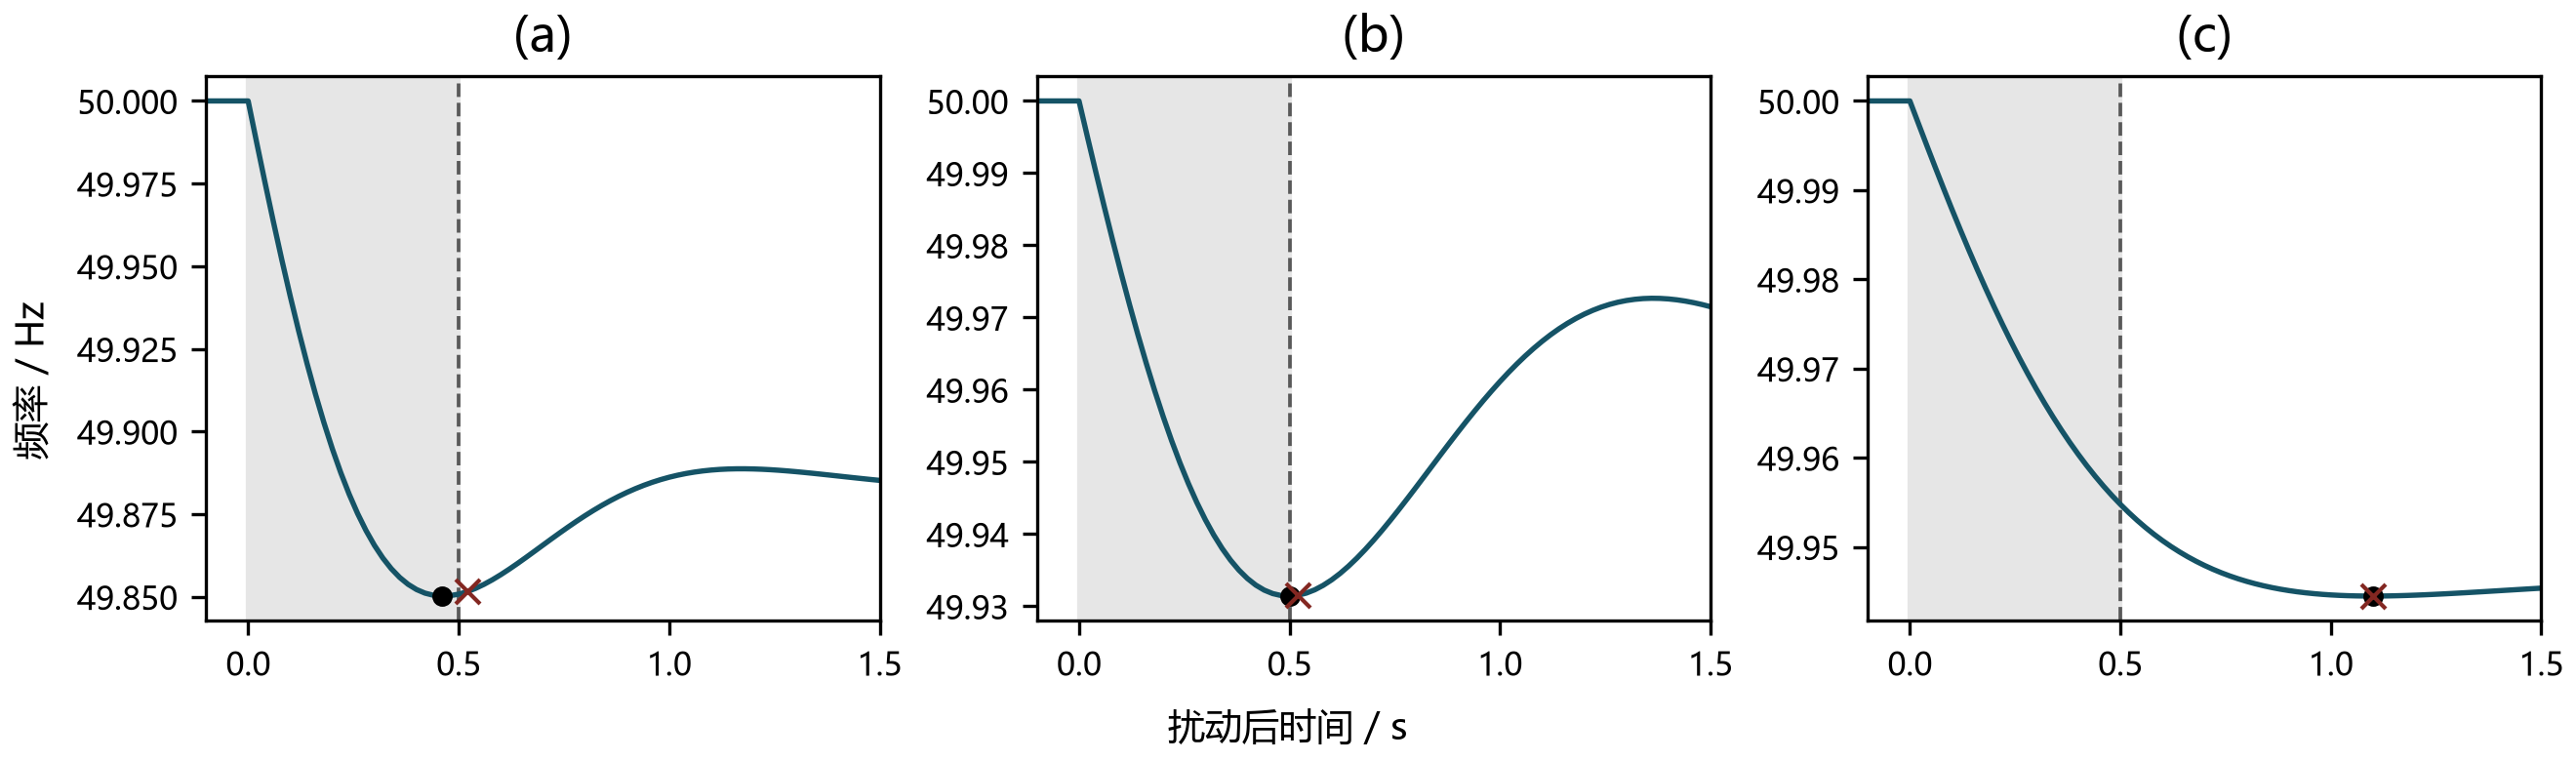
\includegraphics[width=\linewidth]{assets/timeline.png}
\caption{观测窗口与截止后最低频率\quad （a）截止前形成；（b）截止时形成；（c）截止后形成\\
Fig. \thefigure\quad Observation window and subsequent minimum frequency}
\label{fig:timeline}
\end{figure}

图中灰色区为可见窗口，圆点表示全局最低点，叉号表示截止后预测目标。主条件样本提前量的最小值、第5百分位数和中位数分别为\LeadMin{}、\LeadPfive{}和\LeadMedian{} s。这些间隔只反映仿真中的时间余量，尚未扣除扰动检测、数据传输与计算时延。

\section{短窗特征与评价方法}
\subsection{特征构造}
记$a=f(t_c)-f_0$。在本文条件样本的无噪声窗口内，单调下降使得全窗平均斜率和幅度分别为$a/0.50$与$-a$，与端点频偏构成一维信息。低阶物理模型也说明初始变化率主要受$d/H$影响，而后续斜率还会受到阻尼和调频出力变化影响。为比较形状信息，构造如下配置。

\begin{enumerate}
\item 端点频偏及端点与初始变化率的组合。初始变化率取扰动后0至0.10 s的首尾差分。
\item 端点与二次拟合系数组合。在完整窗口上拟合二次多项式，时间缩放至$[0,1]$，保留一次项与二次项系数。
\item 端点与分段斜率组合。在相对扰动时刻0至0.16、0.16至0.32、0.32至0.48 s的3段上分别计算首尾差分斜率，或以段内全部9点拟合直线斜率。0.50 s采样点由端点特征提供。
\item 端点与变分模态分解能量特征组合。对可见窗去均值后进行4模态分解，以4个模态能量占比及能量熵描述形状\cite{vmd}，绝对收敛容差取$10^{-6}$。
\end{enumerate}

首尾差分的误差由两次观测的噪声决定。在线性趋势和独立等方差噪声假设下，最小二乘斜率的噪声方差与$1/\sum_k(t_k-\bar t)^2$成正比。段内拟合从更多采样点估计变化率，可能降低噪声敏感性，同时也可能平滑真实曲率。两种方案通过同一批含噪测试进行比较。

\subsection{端点信息不足与弦线残差}
令$M=2H$，扰动后时间从零起算。对$x(0)=p(0)=0$、正阶跃缺额$d$且初始阶段未触及调频上限的模型，对方程\eqref{eq:model}在扰动右侧求导可得
\begin{equation}
\dot x(0^+)=-\frac{d}{M},\quad \ddot x(0^+)=\frac{Dd}{M^2},\quad
x^{(3)}(0^+)=-\frac{D^2d}{M^3}+\frac{d}{M^2RT_g}.
\end{equation}
初始瞬时曲率体现阻尼作用。在上述初值下，一阶调频环节从三阶项开始影响局部频率展开。令$\tau$为窗口长度，定义标幺频偏的弦线残差$r_\tau(t)=x(t)-(t/\tau)x(\tau)$。在包含所考察短窗的线性调频段内，由扰动右侧的局部展开得到
\begin{equation}
\begin{aligned}
r_\tau(t)={}&\tfrac{1}{2}\ddot x(0^+)(t^2-t\tau)
 +\tfrac{1}{6}x^{(3)}(0^+)(t^3-t\tau^2)+O(\tau^4),\qquad 0\le t\le\tau .
\end{aligned}
\label{eq:chord-residual}
\end{equation}
初始一阶项在弦线残差中消去，阻尼和一阶调频滞后的影响仍在。式\eqref{eq:chord-residual}是短时局部展开，有限窗的二次拟合系数受整个窗口及高阶项影响。本文用它解释形状来源，预测模型沿用原有频率特征。在区间$[a,b]$对摆动方程积分可得
\begin{equation}
\frac{x(b)-x(a)}{b-a}=-\frac{d}{M}-\frac{D}{M}\bar x_{[a,b]}+\frac{1}{M}\bar p_{[a,b]}.
\end{equation}
同一窗口端点约束全窗的净频率变化，各段斜率仍可反映阻尼和调频支撑在窗内的不同分布。图\ref{fig:matched}固定$H=4$ s、$D=1$、$R=0.05$，分别取$T_g=0.20$和0.70 s，并调节第二条轨迹的$d$以匹配0.50 s端点。两条轨迹的端点均约为49.92275 Hz，截止后最低频率分别为49.91095和49.89164 Hz，二者均未触及调频上限。在进一步的三档参考缺额与四档调频时间常数组合中，12组均匹配成功，匹配后截止最低值与各自参考值相差3.4至44.0 mHz，见补充材料。端点匹配过程中同时改变了缺额与调频时间常数，结果说明同端点可对应不同目标。

\begin{figure}[!htbp]
\centering
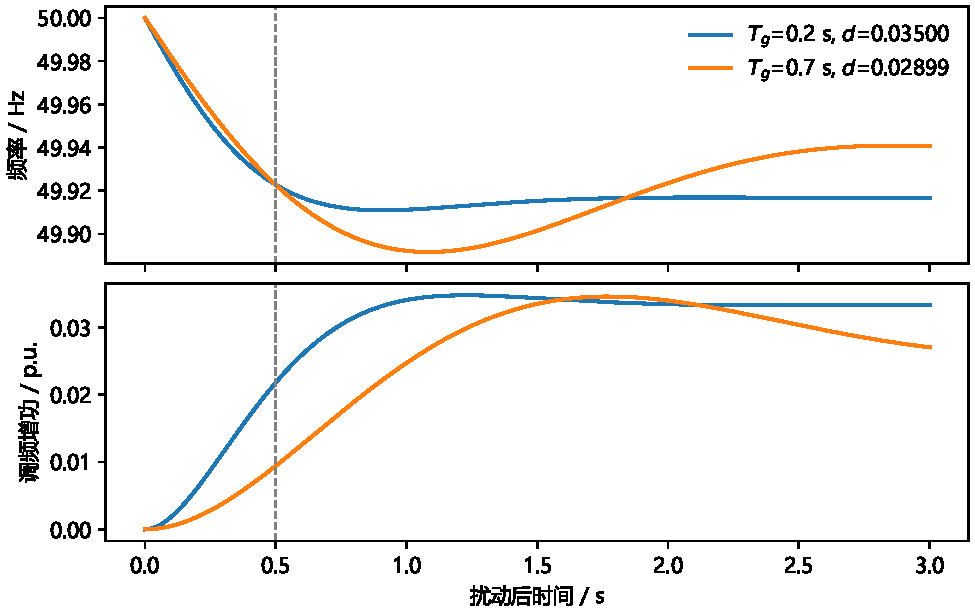
\includegraphics[width=.72\linewidth]{assets/matched-endpoint.pdf}
\caption{端点匹配的频率及调频增功轨迹，虚线表示观测截止时刻}
\label{fig:matched}
\end{figure}

\subsection{未限幅模型的参数等价性}
令$a=d/M$、$b=D/M$、$k=1/(MR)$。在调频指令处于线性段的正阶跃响应中，消去调频增功后得到
\begin{equation}
\ddot x+(b+1/T_g)\dot x+(b+k)x/T_g=-a/T_g,\qquad \dot x(0^+)=-a.
\end{equation}
若保持$T_g$不变，将$H$、$D$、$d$同乘正因子、$R$除以同一因子，上式与初值均保持一致。若两条轨迹均未进入上限饱和或下限截断区，则频率观测无法区分该缩放方向。为估计可见窗中的其他局部方向，对五个对数参数作中心差分，并按模拟白噪声协方差白化。以0.1对数尺度扰动产生至少1单位白化信号为描述性门槛，统计过阈值方向。该门槛用于比较仿真配置，详情见补充材料。

\subsection{模型与划分}
采用持续性基线、岭回归\cite{ridge}及平方损失梯度提升树\cite{friedman}。持续性基线直接使用截止时刻的频率。对$t_n>t_c$的\GridAfter{}个网格场景，以随机种子42划分训练、验证、测试，场景数分别为\TrainN{}、\ValidationN{}、\TestN{}。标准化仅使用训练集统计量。岭回归在验证集上从$10^{-4}$到$10^2$的对数网格选择正则系数，再用训练和验证样本拟合。梯度提升树仅用训练集拟合，树数100，学习率0.1，最大深度3，各特征配置使用相同设置。

扩展测试将46个截止前或截止时事件与\TestN{}个条件测试场景合并，共\FullN{}个未参与训练或选型的场景。该测试特意保留全部46个边界事件，因此合计指标对应此挑战集的构成。以截止后标签小于49.75 Hz定义示例风险事件，报告漏报和误报次数。该阈值用于受控仿真内的误差分析。

\subsection{独立近端点配对协议}
\label{sec:pair-design}
在原训练网格的下垂系数取值之外，预设$R$带$[0.041,0.044]$和$[0.056,0.059]$，每带抽取32个参考场景，各参数在预设范围内独立均匀抽样。每个参考场景分别将$H$、$D$或$T_g$乘以0.8、1.5或1.5，各形成一个候选。每对保留相同的$R$和其余未干预参数，仅在$[0.02,0.08]$ p.u.内调整候选缺额，使干净轨迹的绝对端点差不超过0.10 mHz。原网格训练组拟合标准化器和提升树，验证与历史测试维持原划分。归档近端点扫描只用于开发，正式配对使用独立种子，并检查与历史网格、连续确认、区间试验及开发扫描的参数重合。模型和规则在配对生成前冻结。各候选及其失败原因逐一登记，失败候选不补抽。

四种输入依次为端点、端点＋初始变化率、端点＋二次拟合、端点＋分段拟合。所有配置使用式\eqref{eq:target}及同一0.50 s输入窗。以$B$为候选、$A$为参考，定义
\begin{equation}
\Delta y=y_B-y_A,\qquad \Delta\hat y=\hat y_B-\hat y_A,\qquad
E_\Delta=|\Delta\hat y-\Delta y|.
\label{eq:pair-loss}
\end{equation}
幅度评价纳入可推理且$|\Delta y|\ge 2.00$ mHz的配对，报告$E_\Delta$的平均值（MAE）、均方根值（RMSE）和第95百分位数（P95）。方向评价纳入全部可推理匹配，真值与预测的绝对差各自在0.50 mHz以内或恰为0.50 mHz时计为并列，候选较低、并列、参考较低三个类别一致才计正确。

干净输入为主试验。同批配对另施加30 dB模拟高斯白噪声，每对10个复本。噪声标准差按各成员的干净窗频偏均方根确定。同一成员输入供四模型共用，同一参考的噪声在其候选间复用，两成员噪声独立。MAE变化按待评估模型减基线模型计算。按两个$R$带分层，以参考事件为簇有放回重采样5\,000次，同一参考的候选与复本一起抽取，取2.5和97.5百分位数作为95\%区间。

\subsection{扰动与泛化评估}
噪声实验对干净数据训练得到的固定模型，在测试可见窗加入零均值高斯白噪声。噪声强度以各场景窗内频偏的均方值为基准，在20、30、40 dB分别评估，每档10次独立重复。各配置共享每次重复的噪声样本，标签使用干净轨迹。网格划分敏感性另采用10个随机种子报告均值与标准差。

连续参数验证在表1各参数范围内独立均匀抽样500组，固定预测模型，纳入全部事件类型。惯量外推在$H<6$ s的条件场景训练，留出$H=6$ s的全部240组场景。结构变化检验沿用500组连续参数，将式\eqref{eq:model}的单一调频环节替换为两个串联的一阶环节，时间常数分别为$0.25T_g$和$0.75T_g$，固定其他参数和调频限幅，评估原模型直接迁移的误差。

各实验报告均方根误差、平均绝对误差、绝对误差第95百分位数和决定系数。高斯噪声下按每次重复分别计算指标后取均值。重复划分标准差描述给定样本集上的划分敏感性。

\subsection{端点约束协方差加权的弦线残差估计}
\subsubsection{零端点形状与工作协方差}
为检验式\eqref{eq:chord-residual}中的窗内信息能否形成可用预测表示，构造端点约束的协方差加权弦线残差估计（ECGR）。本小节以 \(f_i\) 表示窗内第 \(i\) 个频率观测（\(f_0\) 在本小节专指窗首观测），\(u_i=i/25\)。弦线扣除算子 \(L\) 在24个内部点计算
\[
r_i=f_i-(1-u_i)f_0-u_i f_{25},\qquad r=Lf .
\]
保留首尾点和全部残差时可通过加回弦线恢复原窗。ECGR进一步将残差压缩至两列零端点基函数
\[
b_1(u)=u(1-u),\qquad b_2(u)=u(1-u)(2u-1).
\]
前者关于窗中点对称，后者反对称。局部二次、三次项扣除弦线后满足 \(u^2-u=-b_1\)、\(u^3-u=-1.5b_1-0.5b_2\)。有限窗系数反映整窗动态，包括高阶响应，不能直接解释为瞬时初始曲率或单独物理参数。

协方差加权最小二乘的基本构造见文献\cite{aitken1936}。首尾量测误差被多个残差共享，因此原频率白噪声也会在残差中产生相关性。保留两端点时，全维弦线残差与原窗可相互重构。预测收益来自施加约束及收缩的整体估计；现有实验未单独识别白化、反对称项和收缩各项的必要性。设工作协方差 \(S=(I+T_\rho)/2\)，其中 \(T_{\rho,ij}=\rho^{|i-j|}\)、\(\rho=0.65\)。定义 \(LL^\top\) 的加权推广 \(LSL^\top=CC^\top\)，取其下三角 Cholesky 因子 \(C\)，令 \(z=C^{-1}Lf\)、\(Z=C^{-1}B\)，\(B\) 为两列基在内部点的取值。

\subsubsection{整窗估计和三次项收缩}
设 \(\tilde\beta=(Z^\top Z)^{-1}Z^\top z\)，令 \(s^2=\|z-Z\tilde\beta\|^2/22\)，\(v\) 为原训练组 \(\tilde\beta_2^2\) 的均值并设置 \(10^{-8}\) Hz$^2$下限。最终系数为
\[
\hat\beta=\arg\min_\beta\bigl\{\|z-Z\beta\|^2+
\lambda(s^2/v)\beta_2^2\bigr\}
=\bigl[Z^\top Z+\operatorname{diag}(0,\lambda s^2/v)\bigr]^{-1}Z^\top z .
\]
\(\lambda\) 从 \(\{0.25,1,4,16\}\) 在历史验证集选为 \ELambda，评分对干净及模拟白噪声的单场景MAE相对二次拟合归一后等权。输出 \(f_{25}-50,\hat\beta_1,\hat\beta_2\)。普通全窗二次拟合采用等权自由截距模型，ECGR还含反对称方向及随窗口变化的收缩。构造测试中，旧二次拟合系数与首尾点完全相同的两个窗口可获得不同ECGR表示。工作协方差为固定估计假设，\(s^2\) 可以含未建模的动态。

窗长固定后离线预计算白化和残差矩阵，稠密分解为 \(O(n^3)\)，存储和单窗计算为 \(O(n^2)\)，\(n=26\)。在线完成两维线性方程求解后调用原提升树。ECGR内部参数、归一尺度和预测模型在后续门控开发和确认中保持冻结，并通过历史预测向量指纹核验。
\begin{figure}[htbp]\centering
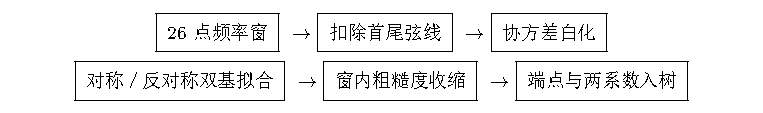
\includegraphics[width=.87\linewidth]{quality-assets/figures/ecgr-flow.pdf}
\caption{ECGR的估计流程。端点同时提供弦线约束和点预测输入。\\Fig. \thefigure\quad Estimation workflow of ECGR}\label{fig:flow}
\end{figure}

\subsection{可观测质量门控}
沿用式\eqref{eq:target}的截止后目标。五种固定点预测器均使用原0.50 s窗；门控另使用扰动前1 s的50点量测判断质量，这些数据仅供选择表示。记扰动前观测均值为 \(m_-\)，去均值均方根为 \(s_-\)，窗内相对 \(m_-\) 的均方根为 \(A\)。定义
\[
Q_-=\frac{s_-}{\max(A,0.005\,\mathrm{Hz})},\quad
Q_w=\frac{\operatorname{RMS}(\Delta^3f)}{\sqrt{20}\max(A,0.005\,\mathrm{Hz})},
\qquad Q=\max(Q_-,Q_w).
\]
白噪声下第三差分滤波的方差倍数为20，相关噪声下此因子只用于尺度归一。开发集比较了扰动前单代理、混合代理、阈值组合及二次或分段作为中间表示。按六条件、两任务归一MAE等权平均，加两倍保护违约惩罚。确定 \(0\le Q\le\GateClean\) 用ECGR，\(\GateClean<Q\le\GateFallback\) 用二次拟合，质量不可用或超过上限时用端点。分段和初始变化率保留为固定对照。端点为开发集选定的跨条件最佳固定策略。噪声类型、真信噪比及截止后真值仅用于仿真或事后评价。

门控开发使用48个配对参考和64个独立单场景。随后保存规则、来源及模型指纹，再用新种子生成最终确认。最终确认样本与训练、开发、原独立配对和ECGR独立确认样本隔离。条件评价沿用式\eqref{eq:pair-loss}的差值误差方向。确认涵盖干净、40/30/20 dB白噪声、同30 dB期望功率的AR(1)（系数0.8），以及扰动时由40 dB白噪声变为20 dB AR(1)的突变。每个含噪条件使用10个复本。主配对幅值评价要求真实差的绝对值至少2 mHz；方向评价纳入全部有效匹配，绝对差不超过0.50 mHz时判为并列。ECGR先在自己的独立确认集验证，使用干净及30 dB模拟白噪声；门控另用新的确认集。各批匹配构造和样本流转见补充材料。两任务分别按事件或参考场景分层聚类重采样5000次。冻结门槛要求两类等条件MAE均改善至少2\%，且变化区间上限低于零。P95保护为各预设对照的105\%，干净参照二次拟合，30 dB参照端点，其余参照最佳固定策略。另检验干净收益保留及30 dB MAE保护。

\subsection{双侧预测区间的独立校准}
以0.50 s二次拟合预测器作附加区间分析。600个开发场景估计误差尺度，另以600个场景校准90\%双侧分割保形区间\cite{angelopoulos2023}，用1200个新场景评估覆盖率及宽度。分组规则与计算式见补充材料。

\section{由后缀预测到滚动告警}\label{sec:rolling-method}
\subsection{共用模型与逐时刻目标}
聚合场景沿用式\eqref{eq:model}的限幅模型。对每个相对决策时刻 $\tau_j\in\{0.20,0.30,0.40,0.50\}$ s，以截至该窗末的量测预测窗末之后的最低频率，沿用式\eqref{eq:target}的严格晚于窗末原则。固定截止试验和滚动试验的各自记录终点、数据与回归器依冻结协议确定。滚动聚合试验的新场景采用四阶龙格库塔法积分，积分步长为5 ms，输出间隔为20 ms，记录扰动后20 s。$H$、$D$、$R$、$T_g$与$d$分别在$[2,6]$ s、$[0.5,2]$、$[0.04,0.06]$、$[0.2,1]$ s与$[0.02,0.08]$范围内独立均匀抽样。

每个决策时刻训练独立的梯度提升回归器，采用100棵最大深度为3的树，预测窗末之后的最低频率。二次拟合模型以窗末频率和归一化窗时间上的一次、二次项系数为输入。持续性基线直接用窗末频率表示后续最低频率。IEEE 39节点高负荷试验另比较跌幅残差模型，该模型用窗末频率减去估计的非负剩余跌幅。二次拟合和残差回归使用既有的1200组聚合开发网格。固定时刻策略只在0.50 s作出判断。

\subsection{事件级校准与时间对齐}
事件级阈值校准从未越限事件控制目标虚警工作点\cite{rigollet}。在各策略的未越限校准事件上，提取可用决策时刻的最小预测值，以其经验分位数选取告警阈值。一个事件只记录首次触发。设$t_a$为告警发出时刻，$t_{\mathrm{cross}}$为参考频率首次严格低于$0.995f_0$的采样时刻。满足$t_a<t_{\mathrm{cross}}$的越限事件计为及时命中，有效提前量为$t_{\mathrm{cross}}-t_a$。在$t_{\mathrm{cross}}$及以后触发计为迟报。及时命中率以全部越限事件为分母，实际虚警率以全部未越限事件为分母，提前量只在及时命中事件中统计。50 Hz聚合算例和60 Hz多机算例的评价阈值分别为49.75 Hz和59.70 Hz。

告警发出时刻取最后一个输入样本可用时刻加设定处理时延。起点偏差改变输入窗的样本位置，以真实扰动时刻为基准的越限时间轴保持一致。多机轨迹使用采样时刻之前最近的已接受积分点。求解诊断中的事后插值仅用于比较积分轨迹。

\subsection{量测质量分级与置信区间}
每个事件用扰动前1 s的50个采样值估计标准差。高低质量分界是按开发集参考频偏确定的40 dB和20 dB噪声标准差的几何均值。固定阈值使用未越限校准事件的全部主量测版本，分级阈值使用相应质量等级内的校准数据。主设置等权合并干净量测、40 dB白噪声、20 dB白噪声和与20 dB白噪声同方差的相关噪声，相关噪声的一阶自回归系数为0.8。噪声加在预警输入，越限判定使用原频率轨迹。同一物理事件的各量测版本在95\%区间估计中随事件一同重采样。

同一低频阈值用于判断事件是否越限，而不同预测策略可有不同校准阈值。固定截止的任务误差衡量频率幅值，滚动的及时命中取决于越限及告警时间。即使点预测误差较小，首次可决策时刻晚于越限仍无法形成及时命中。

\subsection{ECGR质量门控的滚动迁移}\label{sec:roll-transfer}
四个决策时刻0.20、0.30、0.40、0.50 s分别有11、16、21、26点。设某窗有$n$点，$u_j=j/(n-1)$。两个端点与$n-2$个内部点构成弦线矩阵$L$，相应行是$[-(1-u_j),\,\boldsymbol e_j^\mathsf T,\,-u_j]$。$B$在内部点取$u_j(1-u_j)$及$u_j(1-u_j)(2u_j-1)$，$S=(I+\operatorname{Toeplitz}(0.65^{|i-j|}))/2$，$C$为$LSL^\mathsf T$的下三角Cholesky因子。ECGR仍用$\lambda=4$和固定截止原开发尺度$v=7.3831\times10^{-5}$ Hz$^2$；各窗按$n-4$个残差自由度估计窗内尺度，未按窗重估$v$。预测器按窗分别在原1200组开发轨迹上拟合，每个表示用100棵、最大深度3的梯度提升树；特征以Hz及相应斜率单位直接输入，无独立标准化器。

同一次扰动的50点扰动前量测在四窗共用；幅度分母和三阶差分按当前可见窗计算，因此$Q$可随窗长改变。原门槛0.0025、0.016按窗使用，低值选ECGR、中间选二次、高值或不可用退回端点。800个新事件用于告警校准，另以2400个独立事件确认。开发档案截至扰动后19 s，校准和确认截到20 s，均预测窗后的最低频率。对校准和确认的存档参数回放原积分器，经逐窗验证20 s标签后，截短到19 s未改变任何标签；开发档案缺少同求解器的20 s轨迹。

五种主量测（干净、三档白噪声和30 dB等功率AR(1)）等权混合，各策略分别用同一未越限变体校准全局告警阈值；突变不参加校准。10\%目标的门控滚动与二次滚动是预设主要比较，及时命中率差应至少为2个百分点且95\%区间下限大于零，混合和突变虚警增量的区间上限分别不得超过2和5个百分点。5\%为次要工作点；按同一扰动前质量标记分别校准两策略为次要诊断，见补充表\ref{sup:tab:transfer-cutoffs}。区间按物理事件配对重采样，保留各量测变体。

\subsection{最低有效提前量与决策规则的开发}\label{sec:lead-method}
设$T$为真实首次越限时刻，$A$为首次告警时刻。无越限或无告警时，相应时刻取无穷大。给定最低提前量$\ell$，有效命中率和实际虚警率分别以全部越限和未越限的事件—量测组合为分母：
\begin{equation}
 H_\ell=P(A<T,\ T-A\ge\ell\mid T<\infty),\qquad
 F=P(A<\infty\mid T=\infty).
\end{equation}
若首个可决策时刻为$t_1$，则$H_\ell\le P(t_1<T,\ T-t_1\ge\ell\mid T<\infty)$。早越限事件保留在分母中。同一阈值下，增大$\ell$只能减少有效命中，却可能改变两种策略的排序。取$\ell=0$时仍须严格早于越限。

在前一滚动试验的800个校准事件上开发新的决策规则。三个质量区各从四种表示中选一，比较全部64种映射，以至少提前200 ms的有效命中数选定映射。持续性、端点、二次拟合和离散物理库按同一标准竞争简单基线。随后在另800个事件上独立校准各策略阈值并冻结，再在2400个新聚合事件上确认。五种主量测等权，突变单列。200 ms在本次确认前已用于开发，仅表示数值研究设定的最低提前量。

冻结阈值的确认以首次告警计数。另用测试标签构造评分曲线，在5\%和10\%实际虚警率处作等虚警诊断；相同评分同时纳入，相邻可达工作点间线性插值。报告0、100、200和300 ms，0 ms仍须严格早于越限。确认比较按物理事件配对重采样2000次。另以直接输入各窗全部可见频率样本的完整窗树作事后对照，沿用各自冻结阈值，按物理事件配对重采样5000次。

\section{固定截止最低频率预测结果}
\subsection{短窗形状信息的预测收益}
表\ref{tab:main}显示，梯度提升树从单一端点扩展到初始变化率、二次拟合或分段斜率后，误差均下降。二次拟合在干净条件测试的均方根误差最低，为\MainQuadRMSE{} Hz。分段差分与分段拟合分别为\MainSegmentRMSE{} Hz和\MainFitRMSE{} Hz。分段拟合与二次拟合的差距小于端点与任一形状特征的差距，主要收益来自引入早期轨迹形状。岭回归也呈现相同的改善方向。

\begin{table}[!htbp]
\centering\small
\caption{条件测试中的特征与回归器对比\\Table 2\quad Features and regressors on the conditional test set}
\label{tab:main}
\begin{tabular}{llrrrr}
\toprule
特征 & 模型 & 均方根误差/Hz & 平均绝对误差/Hz & 尾部误差/Hz & $R^2$\\
\midrule
\resultrows{revision-assets/main.tex}
\bottomrule
\end{tabular}
\end{table}

在固定0.50 s之后的标签和232个条件测试事件上，图\ref{fig:matrix}对比各窗相对同窗端点的MAE降幅，表\ref{tab:windows}列出端点模型的绝对误差。名义0.25 s窗的实际末样本为0.24 s。0.10 s窗按2、2、1个样本间隔分段，末段仅含两点。

\begin{figure}[!htbp]
\centering
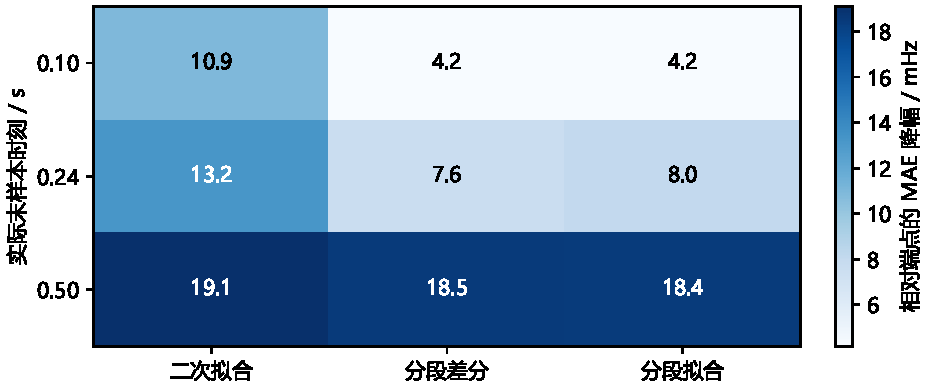
\includegraphics[width=.76\linewidth]{assets/window-gain.pdf}
\caption{固定目标下各观察窗内形状特征相对端点的平均绝对误差降幅}
\label{fig:matrix}
\end{figure}

同一事件内比较各窗形状增益，再按事件重采样。由0.10 s延长至0.50 s时，二次拟合的MAE降幅增加8.2 mHz，95\%区间为$[5.2,11.2]$ mHz；由0.10 s延长至0.24 s的区间跨零。分段配置的跨窗结果见图\ref{fig:matrix}，各窗的分段长度和样本数随窗长变化。

\begin{table}[!htbp]
\centering\small
\caption{固定目标下的观察窗长度比较\\Table 3\quad Observation-window comparison with a fixed target}
\label{tab:windows}
\begin{tabular}{rrrrr}
\toprule
名义窗口/s & 均方根误差/Hz & 平均绝对误差/Hz & 第95百分位数/Hz & $R^2$\\
\midrule
\resultrows{revision-assets/windows.tex}
\bottomrule
\end{tabular}
\end{table}

\subsection{等端点扫描与局部可辨识性}
在36组扩展候选中，35组在规定缺额范围内匹配成功，端点差均小于0.001 mHz。惯量、阻尼和调频时间常数三类扫描的截止后目标绝对差分别为9.1至28.3、0.4至3.6和5.2至32.7 mHz。端点匹配也改变了缺额，这些范围描述相应等端点配对。

从连续参数档案选取60组，其中53组及其差分复本的采样记录均未触及调频上限。在0.50 s及30 dB模拟白噪声下，端点、端点加二次拟合、端点加分段拟合以及完整窗口达到至少两个局部可测方向的场景数分别为0、25、13和34。二次拟合在部分场景多保留一个方向，目标梯度在过阈值方向上的平方投影比例中位数仍与端点接近。40 dB时该二次拟合配置的比例中位数升至99.4\%。该指标衡量局部方向与目标的关系。未限幅的37组参数缩放复核中，最大频率轨迹差约为$4.6\times10^{-11}$ Hz。逐场景结果及步长核查见补充材料。

\subsection{独立近端点配对的幅度与方向结果}
\label{sec:pair-results}
\PairReferences{}个参考场景生成\PairAttempted{}个候选，全部匹配，最大绝对端点差为$\PairMaxEndMantissa\times10^{-10}$ Hz。幅度分析纳入\PairPrimaryPairs{}对，\PairTrueTies{}个真实并列及\PairSmallNonTies{}个小差非并列对全部参加方向评价。所有正式配对成员的全局最低点都在截止后形成。分参数带与排除账本见补充材料。

干净条件下，端点、二次拟合和分段拟合的差值MAE分别为\CleanEndMae{}、\CleanQuadMae{}和\CleanSegMae{} mHz。相对端点，二次拟合和分段拟合的MAE变化分别为\CleanQuadVsEnd{}和\CleanSegVsEnd{} mHz；相对端点＋初始变化率，两者分别为\CleanQuadVsRate{}和\CleanSegVsRate{} mHz。括号内为95\%区间。仅加入初始变化率的变化为\CleanRateVsEnd{} mHz，区间跨零。端点基线把所有干净配对判为并列，只在真实并列时判对，体现了近同端点设计下该基线的行为。

30 dB模拟白噪声下，相对端点，二次拟合的MAE变化为\WhiteQuadVsEnd{} mHz，区间跨零；分段拟合和初始变化率配置分别变化\WhiteSegVsEnd{}和\WhiteRateVsEnd{} mHz，均为增加。二次拟合的差值RMSE和P95为\WhiteQuadRmse{}、\WhiteQuadTail{} mHz，高于端点的\WhiteEndRmse{}、\WhiteEndTail{} mHz。二次拟合与端点的方向判对率分别为\WhiteQuadAcc{}\%和\WhiteEndAcc{}\%，方向判断的提高未伴随差值幅度误差的明确改善。干净与白噪声的方向评价分母分别为\CleanDirections{}和\WhiteDirections{}，白噪声分母按复本计。

\begin{figure}[!htbp]
\centering
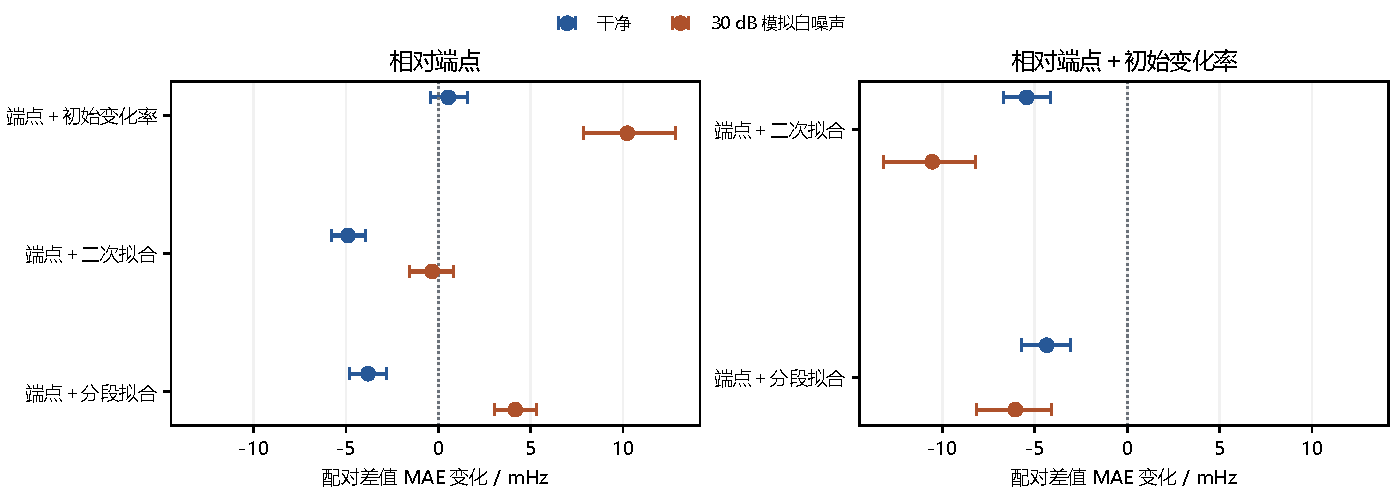
\includegraphics[width=.92\linewidth]{assets/fig-paired-contrasts.pdf}
\caption{近端点配对的差值MAE变化。左侧以端点为基线，右侧以端点＋初始变化率为基线。负值表示待评估模型误差下降，线段为按下垂系数带分层、以参考事件为簇的95\%重采样区间。\\
Fig. \thefigure\quad Changes in MAE of pairwise differences relative to the two baselines}
\label{fig:pair-effects}
\end{figure}
\begin{figure}[!htbp]
\centering
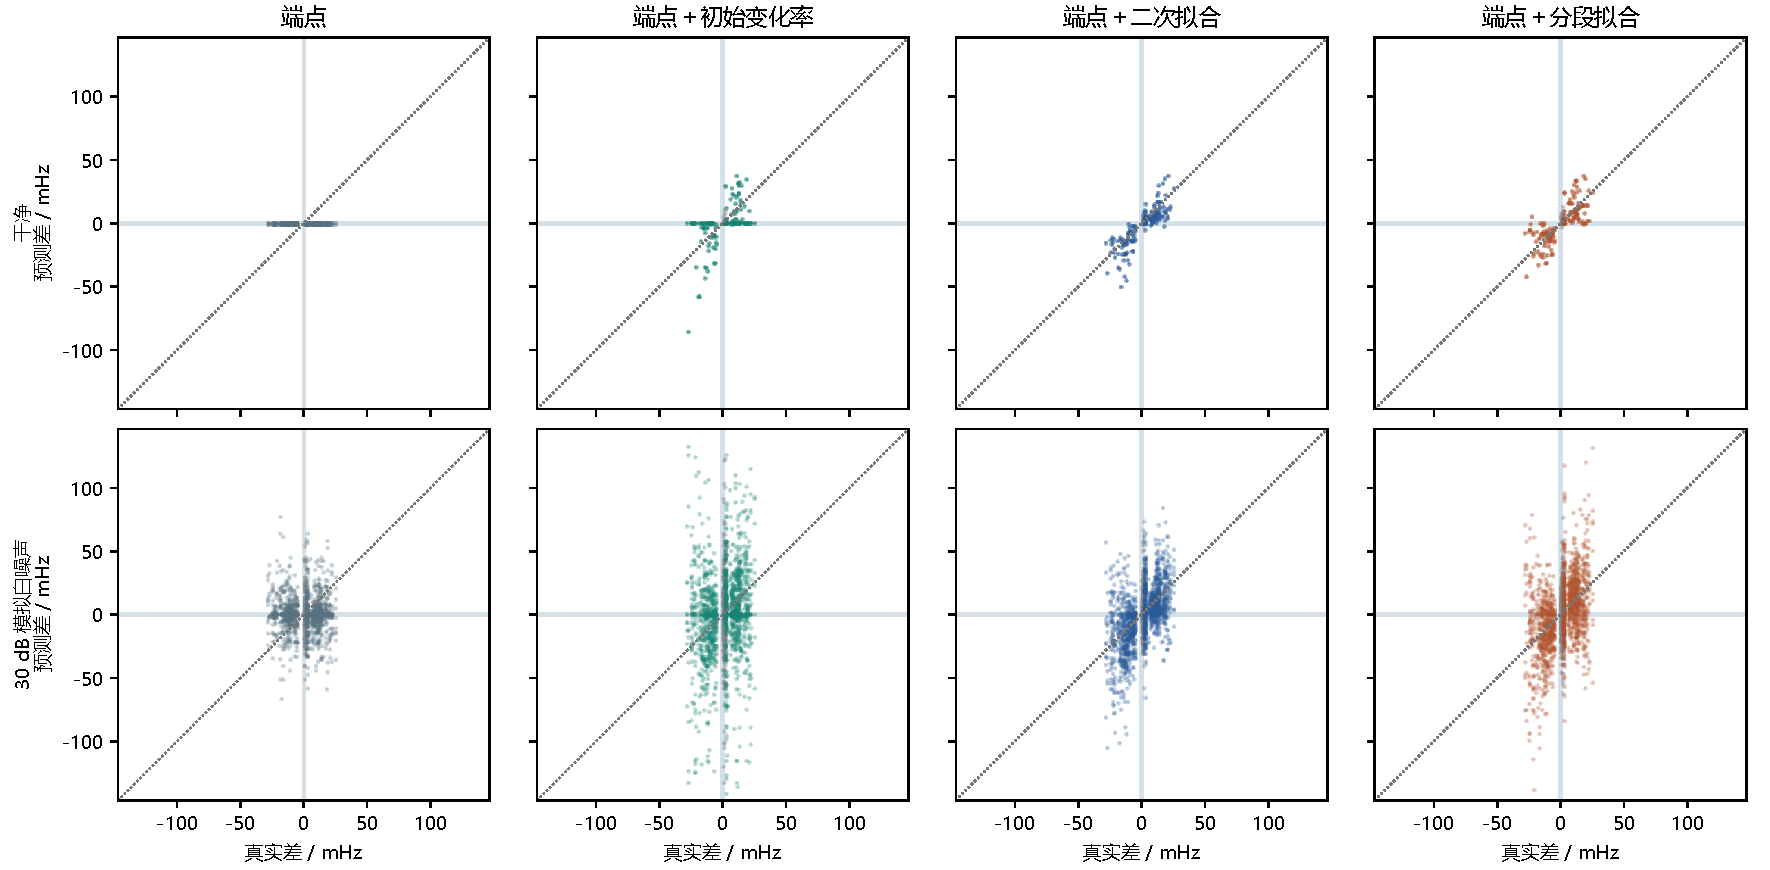
\includegraphics[width=\linewidth]{assets/fig-pair-deltas.pdf}
\caption{近端点配对的最低频率预测差与真实差。横纵轴均为候选减参考。彩点为主幅度评价配对，灰点为其余可推理匹配。淡色横纵带为$\pm0.50$ mHz并列区，虚线为等值线。上排为干净量测，下排为30 dB模拟白噪声下的逐复本结果。\\
Fig. \thefigure\quad Predicted versus true nadir differences for near-endpoint pairs}
\label{fig:pair-deltas}
\end{figure}

图\ref{fig:pair-deltas}给出真值差与预测差的分布，图\ref{fig:pair-effects}汇总相对两条基线的差值MAE变化。
\subsection{边界事件与示例风险阈值}
表\ref{tab:groups}对比分段拟合和持续性基线。将相对全局最低频率的误差分解为截止后标签的预测误差与目标差，即$\hat y-f_{\min}=(\hat y-y)+(y-f_{\min})$。截止前、时、后三组的平均目标差分别为3.94、0.15和约0 mHz。截止前组中，持续性和分段拟合相对截止后标签的RMSE分别为1.5和41.3 mHz。截止时组仅有6个事件，逐场景结果见复现材料。对扩展测试的\FullAlerts{}个示例低频标签，分段拟合和持续性分别将\FullMisses{}和\FullBaselineMisses{}个判断为阈值以上，分段拟合的相反方向错误为\FullFalseAlerts{}次。

\begin{table}[!htbp]
\centering\small
\caption{扩展测试分组误差及示例风险判定\\Table 4\quad Errors and illustrative risk decisions by event group}
\label{tab:groups}
\begin{tabular}{llrrrrr}
\toprule
方法 & 全局最低点 & 场景数 & 均方根误差/Hz & 第95百分位数/Hz & 漏报 & 误报\\
\midrule
\resultrows{revision-assets/groups.tex}
\bottomrule
\end{tabular}
\end{table}

\begin{figure}[!htbp]
\centering
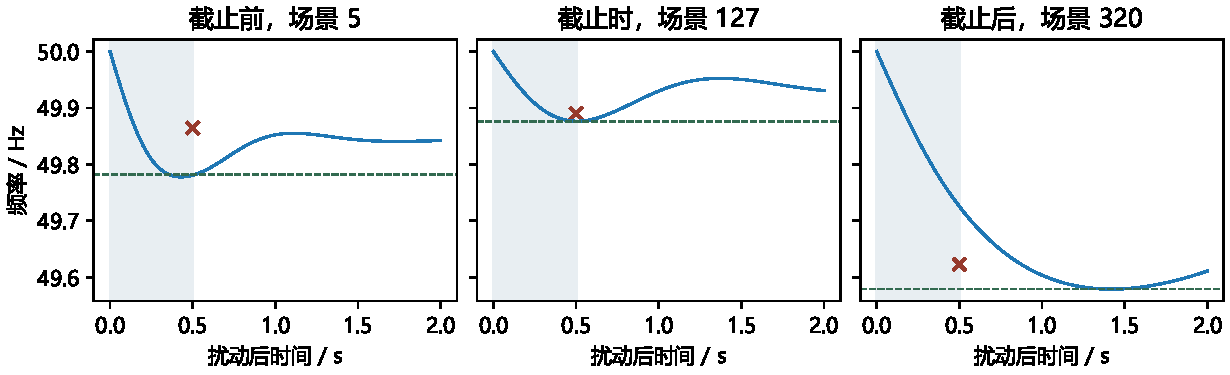
\includegraphics[width=\linewidth]{assets/boundary-cases.pdf}
\caption{三类事件各取分段拟合绝对误差最大的场景。阴影为可见窗，叉号为预测值，水平虚线为截止后目标。}
\end{figure}

\FloatBarrier

\subsection{量测噪声的影响}
如表\ref{tab:noise}及图\ref{fig:noise}所示，端点模型随噪声增强的误差变化较小。20 dB下，分段拟合相比分段差分将均方根误差从\SegNoiseRMSE{} Hz降至\FitNoiseRMSE{} Hz，将尾部误差从\SegNoiseP{} Hz降至\FitNoiseP{} Hz。同一噪声水平下，端点与二次拟合的均方根误差分别为\EndNoiseRMSE{} Hz和\QuadNoiseRMSE{} Hz。在原条件网格的单场景RMSE中，二次拟合在30至40 dB下最低，20 dB下端点最低。该网格结果采用单场景误差，近端点试验采用配对差值误差。短窗形状特征是否值得使用，需由目标量测质量及尾部误差容限共同决定。

\begin{table}[!htbp]
\centering\small
\caption{不同信噪比下的均方根误差与尾部误差\\Table 5\quad Root mean square and 95th-percentile absolute errors under noise}
\label{tab:noise}
\begin{tabular}{lrrr}
\toprule
特征 & 40 dB（Hz） & 30 dB（Hz） & 20 dB（Hz）\\
\midrule
\resultrows{revision-assets/noise.tex}
\bottomrule
\end{tabular}
\end{table}

\begin{figure}[!htbp]
\centering
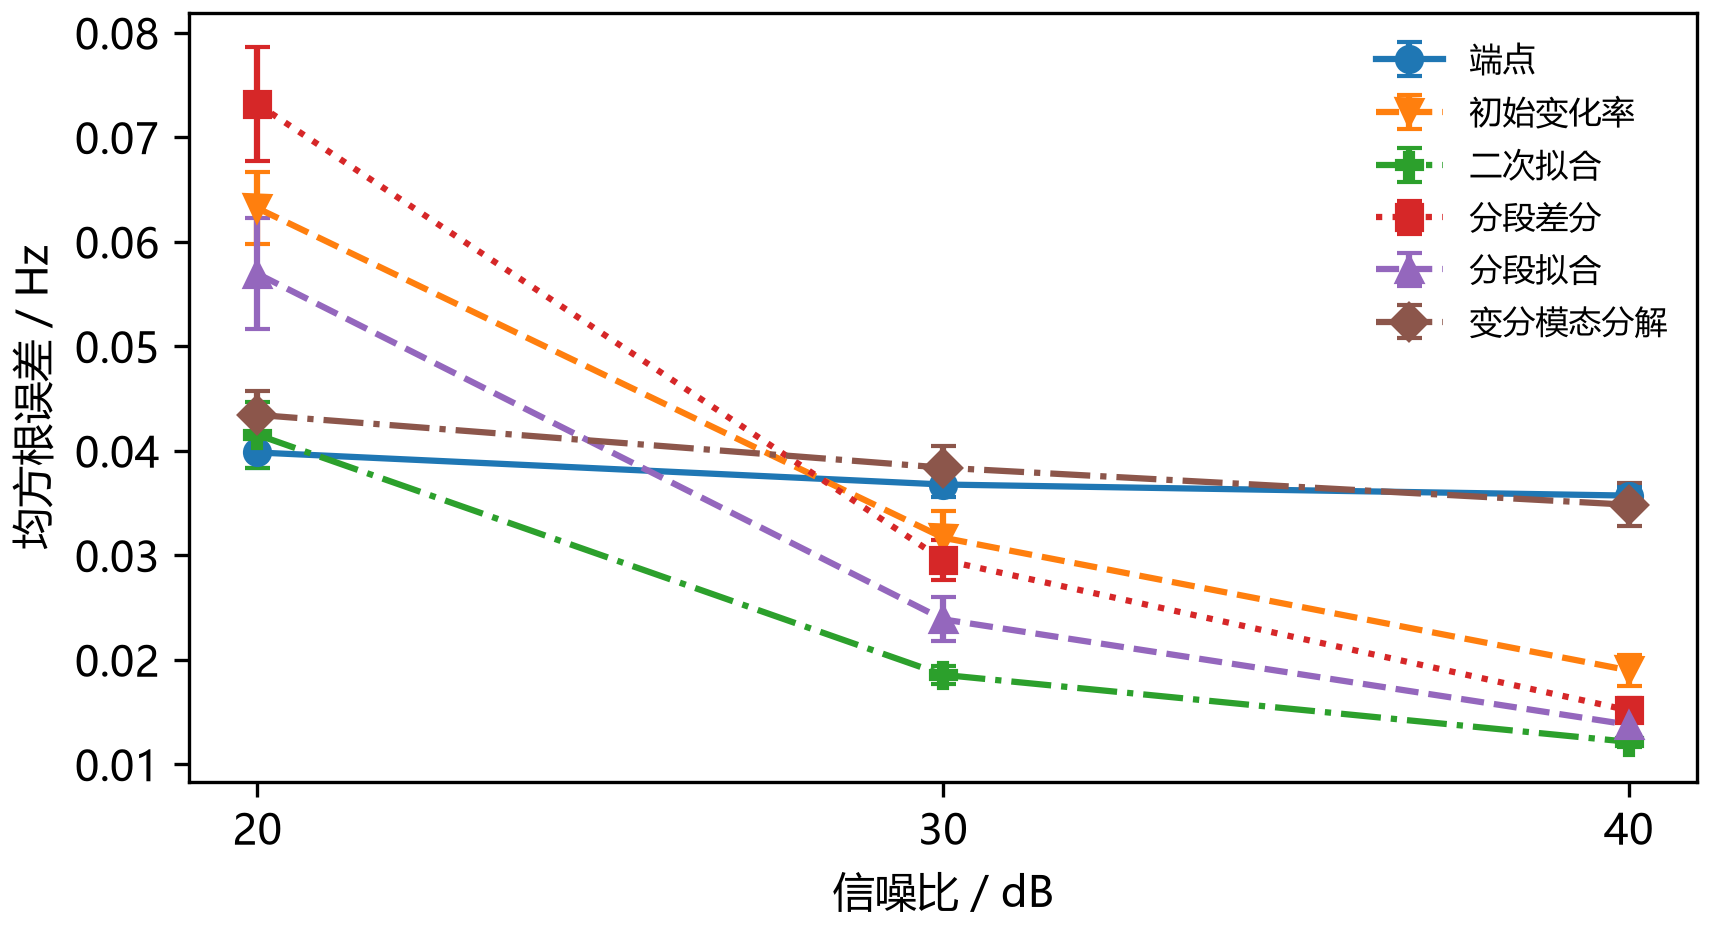
\includegraphics[width=.72\linewidth]{assets/noise.png}
\caption{量测噪声下的均方根误差，误差棒为10次重复的标准差}
\label{fig:noise}
\end{figure}

对同一物理事件内的10个噪声重复取绝对误差差的平均值，再按事件配对重采样。在20 dB下，分段拟合相比分段差分降低MAE 11.3 mHz，95\%区间为[9.5,13.3] mHz；相对端点则增加9.7 mHz，区间为[6.6,12.7] mHz。二次拟合相对端点的MAE降幅为1.7 mHz，区间为[-1.0,4.5] mHz。20 dB下二次拟合的RMSE略高于端点，两种误差指标对个别大误差的权重不同。

另对相同的232个条件场景比较三种全窗期望功率相同的合成噪声，名义全窗信噪比为20 dB。平稳AR(1)噪声的系数为0.8，突变噪声的标准差从0.26 s起提高至早段的3倍，随后统一归一至目标全窗功率。分段拟合相对分段差分的MAE在白噪声和突变噪声下分别降低12.0和14.3 mHz，在相关噪声下增加3.0 mHz，配对95\%区间为[1.9,4.2] mHz。所测噪声的时间结构改变了两种斜率估计的误差排序。各特征的绝对误差和复现条件见补充材料。

\subsection{连续参数、惯量外推与调速器结构变化}
表\ref{tab:general}分别报告连续参数抽样、惯量留出及两级调速器结构测试，三者对应新参数组合、惯量范围外推和结构变化。单级与两级的同参场景配对用于量化结构变化的影响。

\begin{table}[!htbp]
\centering\small
\caption{未见场景和不同调速器结构下的梯度提升树性能\\Table 6\quad Gradient-boosted tree performance in unseen scenarios and with different governor dynamics}
\label{tab:general}
\begin{tabular}{lrrrrrr}
\toprule
 & \multicolumn{2}{c}{连续参数} & \multicolumn{2}{c}{惯量外推} & \multicolumn{2}{c}{两级调速器}\\
特征 & 误差/Hz & $R^2$ & 误差/Hz & $R^2$ & 误差/Hz & $R^2$\\
\midrule
\resultrows{revision-assets/validation.tex}
\bottomrule
\end{tabular}
\end{table}

同参数的500对轨迹中，由单级变为两级后，截止后最低频率平均下降13.6 mHz，分段拟合的平均绝对误差增加8.2 mHz。该变化同时包含输入形状变化与预测目标移动。复现材料分别记录端点变化、扣除端点弦线后的窗内形状变化和目标变化。对按误差变化秩选出的三个案例，补充材料给出调频指令和实际增功。三个案例中，两级结构的增功在响应初期较慢、截止后最低频率较低，且采样记录均未触及调频上限。

十次随机划分结果见补充材料，各划分复用同一原始网格。

\subsection{双侧预测区间的覆盖与宽度}
同分布混合测试中，分尺度区间比统一区间平均窄35.7 mHz，经验覆盖率从92.5\%降至90.5\%；两级调频下分尺度区间仅覆盖79.3\%（表\ref{tab:interval}）。单侧风险下界另有10/21项通过，未满足整体验收条件（补充表\ref{sup:tab:risk-fail}）。

\begin{table}[!htbp]
\centering\small
\caption{固定截止后最低频率的预测区间比较\\Table \thetable\quad Prediction intervals for the post-cutoff minimum frequency}
\label{tab:interval}
\begin{tabular}{lrrrrrr}
\toprule
& \multicolumn{2}{c}{覆盖率/\%} & \multicolumn{2}{c}{平均宽度/mHz} & \multicolumn{2}{c}{下侧漏覆盖/\%}\\
测试条件 & 统一 & 分尺度 & 统一 & 分尺度 & 统一 & 分尺度\\
\midrule
同分布混合 & 92.5 & 90.5 & 152.7 & 117.0 & 1.67 & 2.00\\
两级调频 & 90.0 & 79.3 & 152.7 & 117.5 & 1.25 & 1.33\\
\bottomrule
\end{tabular}
\end{table}

\section{ECGR与质量门控的独立确认}
\label{sec:quality-confirm}
\subsection{固定ECGR的干净增益及噪声边界}
第\ref{sec:pair-results}节检验原二次和分段表示。本节先检验ECGR整体估计，再用另一批场景检验质量门控。ECGR独立确认由\Erefs{}个参考场景形成\Epairs{}对，\Eeligible{}对进入主幅值分析。干净时，ECGR和二次拟合的差值MAE分别为\EcleanMae{}和\QcleanMae{} mHz，差值P95分别为\EcleanTail{}和\QcleanTail{} mHz。相对二次拟合的MAE变化为 \(\Echange\,[\Elow,\Ehigh]\) mHz，括号内为参考事件聚类95\%区间。方向判对为\Edir{}与\Qdir{}，ECGR的方向判对较少。30 dB白噪声下，ECGR相对端点的MAE变化为 \(\EwhiteChange\,[\EwhiteLow,\EwhiteHigh]\) mHz，区间跨零。其P95为\EwhiteTail{} mHz，超过端点的\EndWhiteTail{} mHz及冻结保护线\EwhiteLimit{} mHz。因此，固定ECGR在该阶段的总体验收未通过。图\ref{fig:ecgr}呈现其幅值效应。后续门控保留这一表示，是为了利用干净窗中的收益。
\begin{figure}[htbp]\centering
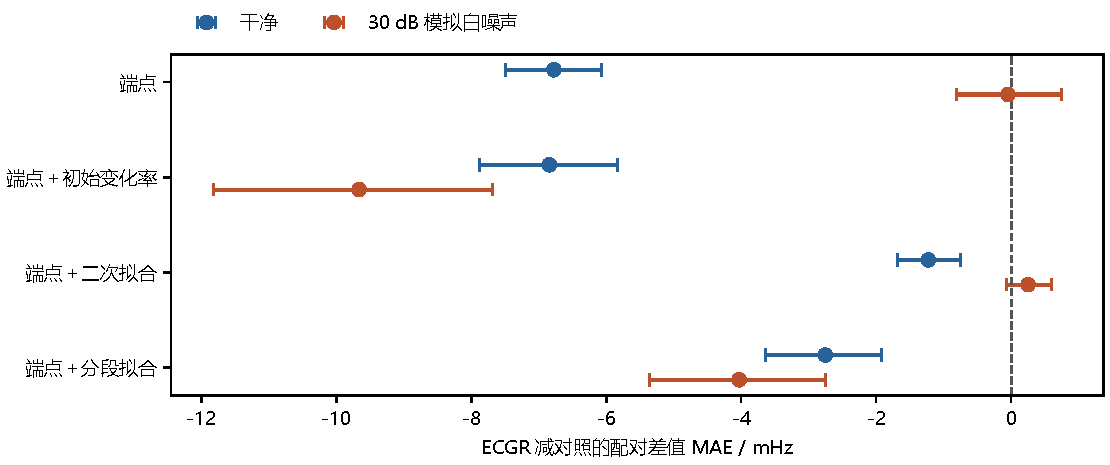
\includegraphics[width=.90\linewidth]{quality-assets/figures/ecgr-paired-contrasts.pdf}
\caption{ECGR独立确认中，相对固定基线的配对MAE变化及聚类95\%区间。负值表示降低。\\Fig. \thefigure\quad Changes in pairwise MAE for ECGR with clustered confidence intervals}\label{fig:ecgr}
\end{figure}

\subsection{同输入对照与估计组件的作用}
在上述已分析过的ECGR确认配对上，重放相同的可见窗和噪声，对附加对照作回顾性分析。采用与原树相同的训练场景和容量，直接输入全部26个频率样本，得到干净配对差值MAE 9.93 mHz。按可见频率窗的最小平方误差从训练参数库中选取物理模型，再用其后缀预测最低点，得到17.29 mHz。完整ECGR为4.44 mHz。物理对照的误差受到候选参数网格间距限制。

分别去除协方差白化、反对称三次项或三次项收缩，三组干净MAE相对完整ECGR的差值区间均跨零。30 dB模拟白噪声下，去白化和去收缩分别使MAE增加5.68和2.15 mHz，去三次项的差值区间仍跨零。完整组合的干净幅值增益不足以证明每一组件均有独立贡献。误差、方向计数及区间见补充表\ref{sup:tab:abl-new}和补充图\ref{sup:fig:abl-new}。

\subsection{门控的平均收益与尾部保护}
质量门控确认集包含\Srefs{}个独立单场景和\Prefs{}个配对参考场景，\Pcount{}个候选全部匹配，\Peligible{}对进入主幅值分析。相对固定端点，等条件单场景MAE从\Sbase{}降至\Sgate{} mHz，降幅\Sgain{}\%，95\%区间为[\Slo{}\%,\Shi{}\%]。配对差值MAE从\Pbase{}降至\Pgate{} mHz，降幅\Pgain{}\%，区间为[\Plo{}\%,\Pupper{}\%]。干净输入全部选用ECGR。30 dB下门控全部退回端点，配对P95为\GateWhiteTail{} mHz，低于\GateWhiteLimit{} mHz保护线；同批固定ECGR为\GateSetEcgrTail{} mHz。全部20项预设门槛通过。图\ref{fig:quality}展示门槛如何对应到选择分布，图\ref{fig:strategy}对照各条件下的主要MAE。 补充图\ref{sup:fig:fixed-q}与图\ref{sup:fig:fixed-errors}给出质量代理和完整基线。
\begin{figure}[htbp]\centering
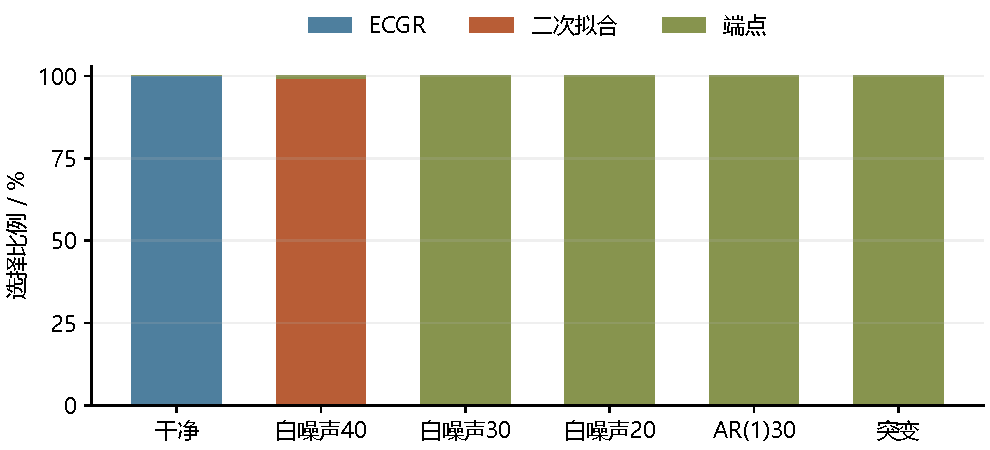
\includegraphics[width=.95\linewidth]{audit-figures/fixed-selection.pdf}
\caption{固定0.50 s门控确认的逐条件表示选择，每柱分母为该条件下独立单事件量测变体。白40、白30、白20表示模拟白噪声信噪比，相关噪声为等功率AR(1)。\\Fig. \thefigure\quad Representation selection by observation condition at the 0.50 s cutoff}\label{fig:quality}
\end{figure}
\begin{figure}[htbp]\centering
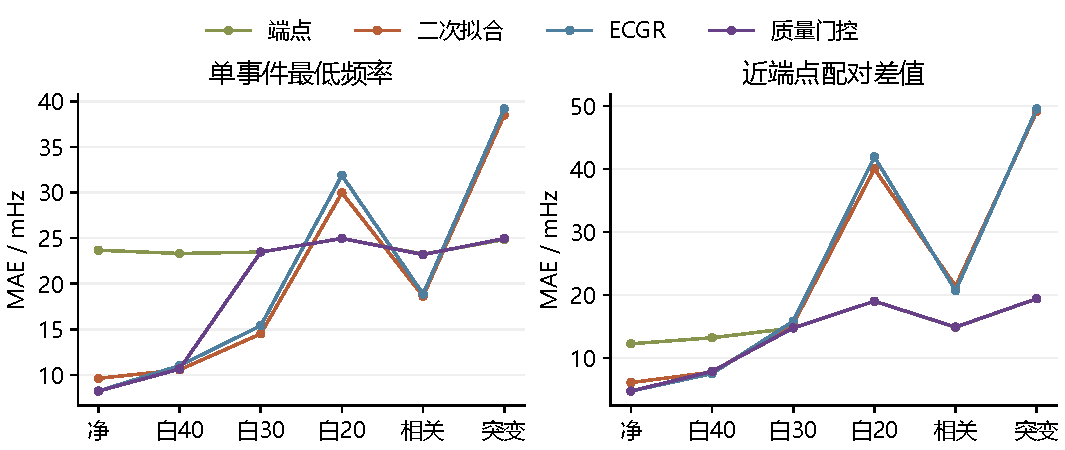
\includegraphics[width=.93\linewidth]{audit-figures/fixed-mae.pdf}
\caption{固定截止门控确认的主要幅值指标。左图为128个独立单事件，右图主幅值集合为220对；含噪各10个复本。全指标及其他基线见补充材料。\\Fig. \thefigure\quad Errors of fixed and gated predictors by observation condition}\label{fig:strategy}
\end{figure}

\subsection{噪声突变与误选}
30 dB下固定二次拟合的单场景MAE为\GateQuadSingle{} mHz，低于门控的\GateWhiteSingle{} mHz。突变时，独立单场景中有\JumpSwitch{}次选用二次拟合，其余退回端点；MAE从\JumpEnd{}升至\JumpGate{} mHz。配对MAE与P95均与端点相同。误选以访问真值后在门控池内逐例取得的最小绝对误差为参照，配对参照允许两成员分别选取表示，等误差不计错。突变单场景和主幅值配对的误选率分别为\JumpSingleMis{}\%和\JumpPairMis{}\%，平均超额误差分别为\JumpSingleLoss{}和\JumpPairLoss{} mHz。该事后参照只用于诊断。补充材料列出混淆矩阵、损失及代表性失败情形。

\section{滚动低频告警的聚合数值试验}
点预测结果说明何时利用短窗形状可以改善幅值估计。本节转向首次越限前能否及时预警，以各自冻结的阈值与事件账本评价，配对差值MAE不作为告警评分。
\subsection{滚动决策与固定时刻决策}
主要对照使用600个校准场景和1600个独立测试场景。291个越限中，98个在0.50 s及以前越限，固定时刻策略的及时命中理论上限为其余193个；实际命中189个，占可及时命中事件的97.93\%。同为5\%校准目标时，滚动在早越限组命中98/98，在晚越限组命中174/193。两者共同命中174个，仅滚动命中98个，仅固定命中15个，均未命中4个。83个净增来自早组增加98个、晚组减少15个，主要体现更早的决策机会。实际虚警为84/1309与74/1309。共同命中事件的中位提前量分别为460和210 ms；全部集合与虚警交集见补充表\ref{sup:tab:original-sets}。固定5\%实际虚警的事后曲线诊断仍显示滚动命中率较高，差27.49个百分点（95\%区间[20.64, 34.01]），见补充表\ref{sup:tab:matched-far}。

\begin{table}[htbp]
\centering
\caption{干净聚合测试的事件级预警结果}\label{tab:r1}
\begin{tabular}{lrrrr}
\toprule
策略 & 及时命中 & 虚警 & 实际虚警率/\% & 中位提前量/ms\\
\midrule
持续性滚动 & 219/291 & 99/1309 & 7.6 & 160\\
二次拟合滚动 & 272/291 & 84/1309 & 6.4 & 390\\
二次拟合固定时刻 & 189/291 & 74/1309 & 5.7 & 240\\
\bottomrule
\end{tabular}
\end{table}

\begin{figure}[htbp]
\centering
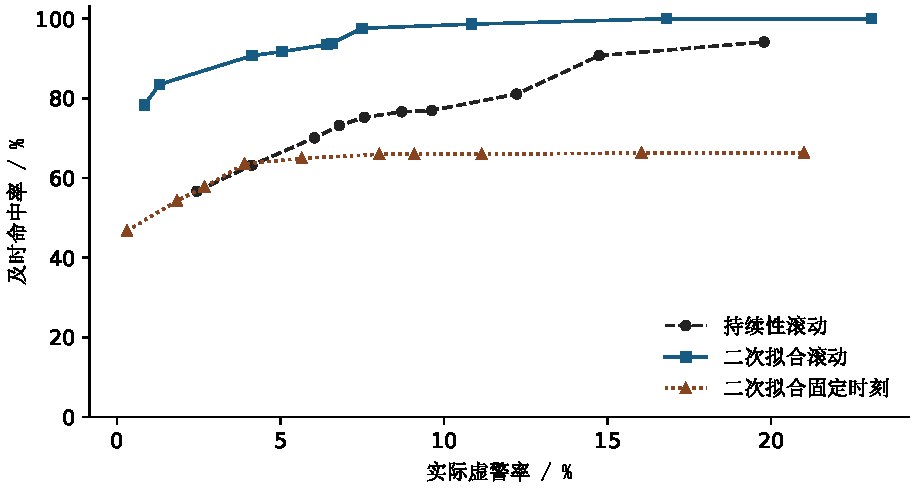
\includegraphics[width=.73\linewidth]{rolling-figures/aggregate-tradeoff.pdf}
\caption{干净聚合试验中不同告警阈值的实际工作点}\label{fig:alarm-tradeoff}
\end{figure}

干净工况的阈值固定后，20 dB量测噪声使滚动二次拟合的虚警升至573/1309，实际虚警率为43.8\%。当20 dB噪声、起点偏晚40 ms及处理时延20 ms同时施加时，虚警达到686/1309，实际虚警率为52.4\%。这说明干净试验的预警工作点对量测条件敏感。

\subsection{混合量测下的分级阈值}
此试验另抽取600个校准场景与1 800个封存物理测试场景，冻结预测模型。每个物理事件在主分析中具有四种量测版本，表中分母统计事件—量测组合，置信区间保留同一事件内的关联。表\ref{tab:r2}以10\%目标虚警设置对照二次拟合固定阈值、分级阈值和持续性分级阈值。相对固定阈值，聚合试验的二次拟合分级阈值提高及时命中率25.2个百分点，按物理事件配对重采样的95\%区间为[22.6, 27.6]个百分点。若量测噪声在扰动时从40 dB突变至20 dB，估计分级的二次拟合达到40.8\%实际虚警率。扰动前标准差对扰动后噪声水平的代表性限制了分级校准的适用性。

\begin{table}[htbp]
\centering
\caption{混合量测下不同阈值方案的封存结果}\label{tab:r2}
\begin{tabular}{llrrrr}
\toprule
算例 & 策略 & 及时命中 & 虚警 & 命中率/\% & 虚警率/\%\\
\midrule
聚合 & 二次拟合固定阈值 & 661/1304 & 610/5896 & 50.7 & 10.3\\
聚合 & 二次拟合分级阈值 & 989/1304 & 542/5896 & 75.8 & 9.2\\
聚合 & 持续性分级阈值 & 1019/1304 & 620/5896 & 78.1 & 10.5\\
IEEE 39节点 & 二次拟合固定阈值 & 17/84 & 20/204 & 20.2 & 9.8\\
IEEE 39节点 & 二次拟合分级阈值 & 48/84 & 25/204 & 57.1 & 12.3\\
IEEE 39节点 & 持续性分级阈值 & 67/84 & 24/204 & 79.8 & 11.8\\
\bottomrule
\end{tabular}
\end{table}

\subsection{ECGR质量门控接入滚动告警的独立试验}
表\ref{tab:transfer-abs}采用同批场景、同一10\%校准目标，各策略分别校准。五条件共享409个越限、1991个未越限物理事件，分别形成2045与9955个量测组合。二次滚动与门控滚动的及时命中率分别为49.49\%和79.32\%，差29.83个百分点（95\%区间[26.46, 33.10]）。实际虚警由912/9955升至1076/9955，差1.65个百分点，区间[0.72, 2.58]。上限2.58超过保护线2个百分点，主验收未通过。表中计数按历史确认程序实际读入的阈值复现，读取精度对并列评分的影响见补充材料。突变时虚警下降6.88个百分点，命中差的区间跨零。提前量仅在各策略自身及时命中集合上取中位数。

同批持续性为新增事后对照。混合条件下持续性命中率81.81\%、虚警率10.41\%，点估计均优于门控；门控减持续性的命中差为−2.49个百分点，区间[−5.41, 0.38]。这组比较不改变预设验收。5\%次要工作点相对二次滚动增加24.35个百分点命中并减少1.57个百分点虚警；它不能替代主要结果。分级阈值诊断相对分级二次滚动的命中差为8.80个百分点，实际虚警差区间[−0.42, 1.18]。各量测条件的实际工作点见补充表\ref{sup:tab:transfer-full}，选择比例与工作点见补充图\ref{sup:fig:transfer-select}和图\ref{sup:fig:transfer-op}。

干净条件下两条混合校准阈值分别为49.65090与49.73574 Hz。阈值交换矩阵的对称分解中，75.79个百分点的命中差有75.55个百分点对应阈值切换，0.24个百分点对应评分切换。它描述该工作点下的代数组成。相同5\%实际虚警的事后插值中，干净条件命中差缩为1.71个百分点，而五条件混合为26.04个百分点。相同实际虚警的诊断以确认数据重建曲线，不代表可部署的阈值选择，见补充表\ref{sup:tab:matched-far}。

\begin{table}[!htbp]\centering\small\setlength{\tabcolsep}{4pt}
\caption{原滚动接入试验的主要对照与持续性参照（10\%校准目标，五种量测等权）。持续性为事后比较，全部策略和突变结果见补充表\ref{sup:tab:transfer-full}。}\label{tab:transfer-abs}
\begin{tabular}{llrrrrrr}
\toprule
量测 & 策略 & 阈值/Hz & 命中/越限 & 虚警/未越限 & 命中/\% & 虚警/\% & 提前/ms \\
\midrule
主条件混合 & 二次滚动 & 49.65090 & 1012/2045 & 912/9955 & 49.49 & 9.16 & 320 \\
主条件混合 & 门控滚动 & 49.73574 & 1622/2045 & 1076/9955 & 79.32 & 10.81 & 260 \\
主条件混合 & 持续性滚动 & 49.82310 & 1673/2045 & 1036/9955 & 81.81 & 10.41 & 180 \\
\bottomrule\end{tabular}\end{table}

\subsection{指定最低提前量下与持续性的比较}\label{sec:new-agg}
开发集选出的最佳简单策略为持续性。按有效命中数选出的三个质量区映射依次为ECGR、二次拟合和端点，与按固定截止幅值误差开发的映射一致。两种门控在新确认集产生相同的评分与首次告警，无法把收益归因于改变了开发目标。2400个新物理事件中401个越限、1999个未越限。五种量测合计2005个越限变体和9995个未越限变体，与前一滚动迁移试验分别计数。

在各自冻结阈值下，要求至少提前200 ms，门控与持续性有效命中1083/2005和758/2005，虚警994/9995和1102/9995。门控的有效命中率高16.21个百分点（95\%区间$[12.28,20.17]$），实际虚警率低1.08个百分点（门控减持续性，$[-2.05,-0.09]$）。突变条件下分别有效命中162/401和156/401，虚警261/1999和221/1999，有效命中率差的区间含零（补充表\ref{sup:tab:abs-new}）。

测试曲线等虚警诊断回答评分排序问题。在10\%实际虚警率下，只要求严格早于越限，门控与持续性的命中率分别为79.27\%和79.43\%；要求至少提前200 ms，两者为54.03\%和32.62\%，差$+21.41$个百分点（95\%区间$[14.19,26.05]$）。四个提前量的结果见图\ref{fig:decision-new}和补充表\ref{sup:tab:roc-new}。

在同批事后对照中，完整窗树与门控的末窗MAE分别为18.90和17.73 mHz，按未舍入逐例误差计算的配对差为$+1.16$ mHz（95\%区间$[0.79,1.55]$）。按两者各自冻结的阈值，完整窗树减门控的200 ms有效命中率差为$+2.84$个百分点（$[-0.30,5.87]$），虚警率差为$-0.47$个百分点（$[-1.16,0.18]$）。仅完整窗树和仅门控满足提前量的分别有405和348个组合。较低的门控末窗误差未形成确定的四窗告警优势（补充表\ref{sup:tab:raw-paired}）。在10\%实际虚警率的测试曲线上，完整窗树的200 ms有效命中率点估计为56.86\%。

\section{IEEE 39节点数值压力检验}
\subsection{阈值校准与高负荷外推}
多机时域试验采用ANDES 2.0的IEEE 39节点动态算例\cite{cui}。以惯量中心频率判定越限，以节点1、20和39的频率均值为预警输入。在同系统校准和测试负荷分离的量测质量试验中，72个测试事件产生288个量测组合，二次拟合应用分级阈值后及时命中率上升，实际虚警率由9.8\%升至12.3\%（表\ref{tab:r2}）。

高负荷外推试验沿用独立校准块已冻结的分级阈值。校准块负荷倍率为0.956、0.982、1.018和1.044，高负荷块使用1.052至1.075之间的八档负荷，保持两类已见扰动位置组合，提高较深阶跃的抽样比例。共预设128个物理场景，118个收敛，70个发生越限。表\ref{tab:r3}给出10\%目标虚警设置结果。相对持续性，二次拟合和残差模型的及时命中率分别低34.3和10.4个百分点，配对95\%区间分别为[28.2, 40.6]和[6.3, 14.6]个百分点。每个收敛场景有四种量测版本，表中的280与192分别对应70个越限事件与48个未越限事件。各方法的实际虚警率不同，表中是预设阈值下的比较。

\begin{table}[htbp]
\centering
\caption{高负荷外推试验的冻结阈值结果}\label{tab:r3}
\begin{tabular}{lrrrrr}
\toprule
策略 & 及时命中 & 虚警 & 命中率/\% & 虚警率/\% & 中位提前量/ms\\
\midrule
持续性 & 242/280 & 9/192 & 86.4 & 4.7 & 1310\\
二次拟合 & 146/280 & 24/192 & 52.1 & 12.5 & 1340\\
跌幅残差 & 213/280 & 23/192 & 76.1 & 12.0 & 1320\\
\bottomrule
\end{tabular}
\end{table}

\subsection{未见扰动位置}
两个未见四母线扰动组合共预设48个场景。16个低幅阶跃场景收敛，且均未越限。32个较深阶跃提前中止。在16个可评分场景的64个量测组合中，持续性、二次拟合和跌幅残差模型分别产生1、3和3次虚警。及时命中率在该批次无法估计。补充材料记录了步长复算、不同积分方法交叉核查、独立潮流筛查和单独实现时间推进的复算。对提前中止且未观察到越限的场景，完整事件的风险状态保留为未知。

\subsection{聚合门控直接迁移的高负荷压力检验}
另在表\ref{tab:r3}的118个收敛事件上回放第\ref{sec:new-agg}节的聚合策略。三个节点的平均频率换算至50 Hz等值尺度作为输入，惯量中心频率按相同标幺阈值判定风险。每个事件使用与新聚合确认一致的五种主模拟量测，产生350个越限、240个未越限变体。表\ref{tab:r3}采用多机校准和四种量测。两个比较共享物理轨迹，直接迁移试验属于已查看场景上的回顾性检验。

沿用聚合校准阈值时，门控与持续性均无触发。对齐测试曲线10\%实际虚警率并要求提前200 ms时，门控有效命中率为52.86\%，持续性为100.00\%，差值为\(-47.14\)个百分点（95\%区间$[-57.23, -37.22]$）。前者揭示阈值迁移失效，后者表明在已完成轨迹上重新对齐工作点也未恢复门控的排序优势。10个未收敛场景的完整风险状态未知。
\begin{figure}[!htbp]\centering
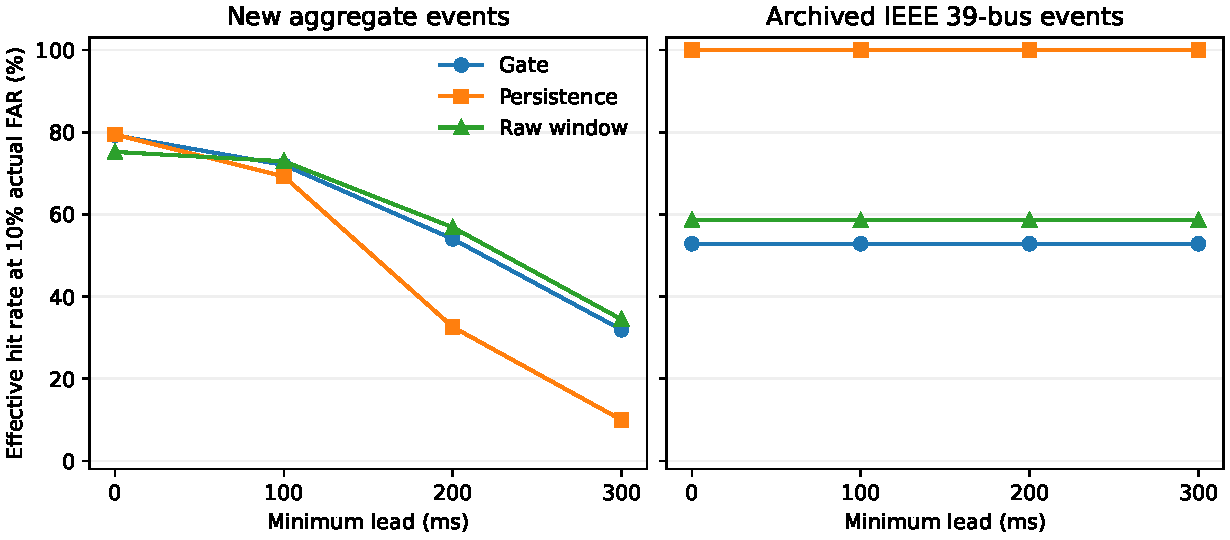
\includegraphics[width=.96\linewidth]{decision-assets/decision-comparison.pdf}
\caption{测试曲线等虚警诊断。各点使用测试标签在10\%实际虚警率处插值，分母为全部越限的事件—量测组合。图例Raw window表示完整窗树。左图为新聚合确认集，右图为已收敛的118个多机高负荷事件的回顾性检验；各自冻结阈值下的整数计数见补充表\ref{sup:tab:abs-new}。}\label{fig:decision-new}
\end{figure}

\section{讨论与适用范围}
等端点约束固定了窗口内的净频率变化，却允许调频支撑在各段有不同的时间分布。弦线残差保留曲线偏离直线的方式，低阶约束及加权估计决定哪些形状成分进入预测。干净配对中二次拟合和分段拟合均提供了端点与所测初始变化率之外的预测信息。正式配对均属截止后形成最低点的场景，主幅值集合以惯量与调频时间常数变化为主。有限窗系数混合多个动态效应，参数缩放等价性限制了单个物理参数的识别。

量测质量改变了值得保留的形状细节。固定ECGR在干净配对上进一步降低差值MAE，同时减少方向判对，30 dB下未通过尾部保护。去组件诊断显示协方差加权和收缩在所测白噪声下有益，尚无足够证据断言反对称三次项必不可少。固定截止质量门控在六条件等权评价中降低单场景与配对误差并通过20项验收，30 dB下固定二次拟合仍可取得更低单场景MAE。突变会削弱观测质量代理的代表性。两级调频下的点预测和区间覆盖压力结果限定了结构迁移的适用范围。

早时刻提供了更多告警机会：原滚动试验对早越限事件多命中98个，对晚越限事件少命中15个。干净条件下的阈值交换还说明，两种策略各用自己的阈值时，命中差可主要来自阈值的位置。新聚合确认中，门控在200 ms冻结工作点较持续性多命中325个组合、少虚警108个；完整窗树与门控的事后对照则显示，末窗幅值误差和四窗首报可给出不同的点估计排序。多机直接迁移时，两种策略均无触发，测试曲线重新对齐虚警率后持续性占优。测点、负荷和系统动态同时改变，现有结果无法分辨各因素对排序反转的贡献。

结论限于所设数值模型、参数、测点及模拟量测。多机比较以求解完成的轨迹为条件，未见扰动位置批次缺少可评分的越限事件。200 ms只表示数值研究指定的最低提前量，现场扰动检测、通信、装置处理和实际控制动作的联合时限仍待独立量测。

\section{结论}
在所设聚合模型中，窗末端点不能唯一确定截止后最低频率。独立近端点配对显示，干净短窗的二次和分段形状可改善差值预测；这一增益受量测质量约束。固定ECGR改善干净配对幅值，但在30 dB白噪声下未通过尾部保护。质量门控相对固定端点降低了指定量测混合下的平均幅值误差。

在新聚合确认的五种主量测中，各自冻结阈值后，门控相对持续性提高了至少提前200 ms的有效命中率，并降低了实际虚警率。原滚动接入试验相对二次滚动的10\%主比较仍未通过虚警保护。事后完整窗树对照未确立门控的四窗告警优势；在已归档的IEEE 39节点高负荷轨迹上，聚合阈值直接迁移失效，按相同实际虚警率比较时持续性占优。短窗形状的预警价值应结合比较对象、所需提前量和阈值适用范围判断。

\noindent\textbf{数据与代码可用性：} 配套材料提供各批冻结配置、场景和状态账本、逐场景及逐配对预测、滚动逐事件评分、数值求解诊断、负面结果与复算索引。配套脚本 \texttt{replay.py} 从归档轨迹、成员预测、逐窗评分及首报复算六项结果；\texttt{compare\_raw.m} 以校准锁和逐窗评分生成完整窗树与门控的配对区间。

\begin{thebibliography}{99}
\small
\setlength{\itemsep}{0pt}
\interlinepenalty=10000
\bibitem{wang2023} 汪梦军，郭剑波，马士聪，等. 新能源电力系统暂态频率稳定分析与调频控制方法综述[J]. 中国电机工程学报，2023，43(5)：1672–1694.\\
WANG Mengjun, GUO Jianbo, MA Shicong, et al. Review of transient frequency stability analysis and frequency regulation control methods for renewable power systems[J]. Proceedings of the CSEE, 2023, 43(5): 1672–1694. DOI: 10.13334/j.0258-8013.pcsee.221466.
\bibitem{sun2020} 孙华东，王宝财，李文锋，等. 高比例电力电子电力系统频率响应的惯量体系研究[J]. 中国电机工程学报，2020，40(16)：5179–5191.\\
SUN Huadong, WANG Baocai, LI Wenfeng, et al. Research on inertia system of power system with high penetration electronics[J]. Proceedings of the CSEE, 2020, 40(16): 5179–5191. DOI: 10.13334/j.0258-8013.pcsee.200493.
\bibitem{dai2026} 代瑞，郭成，张轩. 计及新能源和直流频率限制控制器的最小惯量需求评估方法[J]. 电力系统及其自动化学报，2026，38(9)：112–122. DOI: 10.19635/j.cnki.csu-epsa.001762.\\
DAI Rui, GUO Cheng, ZHANG Xuan. Method for evaluating minimum inertia requirements considering new energy and DC frequency limit controllers[J]. Proceedings of the CSUEPSA, 2026, 38(9): 112–122.
\bibitem{anderson1990} ANDERSON P M, MIRHEYDAR M. A low-order system frequency response model[J]. IEEE Transactions on Power Systems, 1990, 5(3): 720–729. DOI: 10.1109/59.65898.
\bibitem{liu2020} LIU L, LI W, BA Y, et al. An analytical model for frequency nadir prediction following a major disturbance[J]. IEEE Transactions on Power Systems, 2020, 35(4): 2527–2536. DOI: 10.1109/TPWRS.2019.2963706.
\bibitem{zhao2025} ZHAO Z, XUE Y, CHU Z, et al. Generic low-order primary frequency response model for frequency nadir prediction[J]. IEEE Transactions on Power Systems, 2025, 40(6): 5221–5236. DOI: 10.1109/TPWRS.2025.3558912.
\bibitem{luo2019} 罗启珩，王晓茹，刘金强，等. 基于调速系统等值模型的电力系统发生扰动后最低频率预测[J]. 电力自动化设备，2019，39(10)：163–167.\\
LUO Qiheng, WANG Xiaoru, LIU Jinqiang, et al. Minimum frequency prediction of power system after disturbance based on equivalent model of governor system[J]. Electric Power Automation Equipment, 2019, 39(10): 163–167.
\bibitem{wang2018} 王琦，李峰，汤奕，等. 基于物理-数据融合模型的电网暂态频率特征在线预测方法[J]. 电力系统自动化，2018，42(19)：1–9.\\
WANG Qi, LI Feng, TANG Yi, et al. On-line prediction method of transient frequency characteristics for power grid based on physical-statistical model[J]. Automation of Electric Power Systems, 2018, 42(19): 1–9.
\bibitem{li2021} 李冠争，李斌，王帅，等. 基于特征选择和随机森林的电力系统受扰后动态频率预测[J]. 电网技术，2021，45(7)：2492–2502.\\
LI Guanzheng, LI Bin, WANG Shuai, et al. Dynamic frequency prediction of power system post-disturbance based on feature selection and random forest[J]. Power System Technology, 2021, 45(7): 2492–2502. DOI: 10.13335/j.1000-3673.pst.2021.0027.
\bibitem{zhang2025} 张国斌，沈烨昱，霍红岩，等. 基于电力系统受扰后频率最低点预测的一次调频优化研究[J]. 太阳能学报，2025，46(5)：89–98.\\
ZHANG Guobin, SHEN Yeyu, HUO Hongyan, et al. Research on optimization of primary frequency regulation based on frequency nadir prediction after power system disturbances[J]. Acta Energiae Solaris Sinica, 2025, 46(5): 89–98. DOI: 10.19912/j.0254-0096.tynxb.2023-2099.
\bibitem{zhang2019} 仉怡超，闻达，王晓茹，等. 基于深度置信网络的电力系统扰动后频率曲线预测[J]. 中国电机工程学报，2019，39(17)：5095–5104，5290.\\
ZHANG Yichao, WEN Da, WANG Xiaoru, et al. A method of frequency curve prediction based on deep belief network of post-disturbance power system[J]. Proceedings of the CSEE, 2019, 39(17): 5095–5104, 5290.
\bibitem{lu2024} 陆文安，朱清晓，李兆伟，等. 基于卷积神经网络的新型电力系统频率特性预测方法[J]. 上海交通大学学报，2024，58(10)：1500–1512.\\
LU Wenan, ZHU Qingxiao, LI Zhaowei, et al. A prediction method of new power system frequency characteristics based on convolutional neural network[J]. Journal of Shanghai Jiao Tong University, 2024, 58(10): 1500–1512. DOI: 10.16183/j.cnki.jsjtu.2023.071.
\bibitem{li2024fusion} LI H, WANG L, QI S, et al. Power system frequency nadir prediction based on data-driven and power-frequency polynomial fitting[J]. Frontiers in Energy Research, 2024, 12: 1501181. DOI: 10.3389/fenrg.2024.1501181.
\bibitem{chamorro2021} CHAMORRO H R, ORJUELA-CAÑÓN A D, GANGER D, et al. Data-driven trajectory prediction of grid power frequency based on neural models[J]. Electronics, 2021, 10(2): 151. DOI: 10.3390/electronics10020151.
\bibitem{vmd} DRAGOMIRETSKIY K, ZOSSO D. Variational mode decomposition[J]. IEEE Transactions on Signal Processing, 2014, 62(3): 531–544. DOI: 10.1109/TSP.2013.2288675.
\bibitem{ridge} HOERL A E, KENNARD R W. Ridge regression: biased estimation for nonorthogonal problems[J]. Technometrics, 1970, 12(1): 55–67. DOI: 10.1080/00401706.1970.10488634.
\bibitem{friedman} FRIEDMAN J H. Greedy function approximation: a gradient boosting machine[J]. Annals of Statistics, 2001, 29(5): 1189–1232. DOI: 10.1214/aos/1013203451.
\bibitem{angelopoulos2023} ANGELOPOULOS A N, BATES S. Conformal prediction: a gentle introduction[J]. Foundations and Trends in Machine Learning, 2023, 16(4): 494–591. DOI: 10.1561/2200000101.
\bibitem{rietveld} RIETVELD G, WRIGHT P S, ROSCOE A J. Reliable rate-of-change-of-frequency measurements: Use cases and test conditions[J]. IEEE Transactions on Instrumentation and Measurement, 2020, 69(9): 6657--6666. DOI: 10.1109/TIM.2020.2986069.
\bibitem{rigollet} RIGOLLET P, TONG X. Neyman-Pearson classification under a strict constraint[C]//Proceedings of the 24th Annual Conference on Learning Theory. PMLR, 2011, 19: 595--614. \url{https://proceedings.mlr.press/v19/rigollet11a.html}.
\bibitem{cui} CUI H, LI F, TOMSOVIC K. Hybrid symbolic-numeric framework for power system modeling and analysis[J]. IEEE Transactions on Power Systems, 2021, 36(2): 1373--1384. DOI: 10.1109/TPWRS.2020.3017019.
\bibitem{aitken1936} AITKEN A C. IV.—On least squares and linear combination of observations[J]. Proceedings of the Royal Society of Edinburgh, 1936, 55: 42--48. DOI: 10.1017/S0370164600014346.

\end{thebibliography}
\end{document}
